\documentclass{article} % For LaTeX2e
\usepackage{iclr2025_conference,times}

% Optional math commands from https://github.com/goodfeli/dlbook_notation.
%%%%% NEW MATH DEFINITIONS %%%%%

\usepackage{amsmath,amsfonts,bm}
\usepackage{hyperref}       % hyperlinks



% Mark sections of captions for referring to divisions of figures
\newcommand{\figleft}{{\em (Left)}}
\newcommand{\figcenter}{{\em (Center)}}
\newcommand{\figright}{{\em (Right)}}
\newcommand{\figtop}{{\em (Top)}}
\newcommand{\figbottom}{{\em (Bottom)}}
\newcommand{\captiona}{{\em (a)}}
\newcommand{\captionb}{{\em (b)}}
\newcommand{\captionc}{{\em (c)}}
\newcommand{\captiond}{{\em (d)}}

% Highlight a newly defined term
\newcommand{\newterm}[1]{{\bf #1}}


% Figure reference, lower-case.
\def\figref#1{figure~\ref{#1}}
% Figure reference, capital. For start of sentence
\def\Figref#1{Figure~\ref{#1}}
\def\twofigref#1#2{figures \ref{#1} and \ref{#2}}
\def\quadfigref#1#2#3#4{figures \ref{#1}, \ref{#2}, \ref{#3} and \ref{#4}}
% Section reference, lower-case.
\def\secref#1{section~\ref{#1}}
% Section reference, capital.
\def\Secref#1{Section~\ref{#1}}
% Reference to two sections.
\def\twosecrefs#1#2{sections \ref{#1} and \ref{#2}}
% Reference to three sections.
\def\secrefs#1#2#3{sections \ref{#1}, \ref{#2} and \ref{#3}}
% Reference to an equation, lower-case.
\def\eqref#1{equation~\ref{#1}}
% Reference to an equation, upper case
\def\Eqref#1{Equation~\ref{#1}}
% A raw reference to an equation---avoid using if possible
\def\plaineqref#1{\ref{#1}}
% Reference to a chapter, lower-case.
\def\chapref#1{chapter~\ref{#1}}
% Reference to an equation, upper case.
\def\Chapref#1{Chapter~\ref{#1}}
% Reference to a range of chapters
\def\rangechapref#1#2{chapters\ref{#1}--\ref{#2}}
% Reference to an algorithm, lower-case.
\def\algref#1{algorithm~\ref{#1}}
% Reference to an algorithm, upper case.
\def\Algref#1{Algorithm~\ref{#1}}
\def\twoalgref#1#2{algorithms \ref{#1} and \ref{#2}}
\def\Twoalgref#1#2{Algorithms \ref{#1} and \ref{#2}}
% Reference to a part, lower case
\def\partref#1{part~\ref{#1}}
% Reference to a part, upper case
\def\Partref#1{Part~\ref{#1}}
\def\twopartref#1#2{parts \ref{#1} and \ref{#2}}

\def\ceil#1{\lceil #1 \rceil}
\def\floor#1{\lfloor #1 \rfloor}
\def\1{\bm{1}}
\newcommand{\train}{\mathcal{D}}
\newcommand{\valid}{\mathcal{D_{\mathrm{valid}}}}
\newcommand{\test}{\mathcal{D_{\mathrm{test}}}}

\def\eps{{\epsilon}}


% Random variables
\def\reta{{\textnormal{$\eta$}}}
\def\ra{{\textnormal{a}}}
\def\rb{{\textnormal{b}}}
\def\rc{{\textnormal{c}}}
\def\rd{{\textnormal{d}}}
\def\re{{\textnormal{e}}}
\def\rf{{\textnormal{f}}}
\def\rg{{\textnormal{g}}}
\def\rh{{\textnormal{h}}}
\def\ri{{\textnormal{i}}}
\def\rj{{\textnormal{j}}}
\def\rk{{\textnormal{k}}}
\def\rl{{\textnormal{l}}}
% rm is already a command, just don't name any random variables m
\def\rn{{\textnormal{n}}}
\def\ro{{\textnormal{o}}}
\def\rp{{\textnormal{p}}}
\def\rq{{\textnormal{q}}}
\def\rr{{\textnormal{r}}}
\def\rs{{\textnormal{s}}}
\def\rt{{\textnormal{t}}}
\def\ru{{\textnormal{u}}}
\def\rv{{\textnormal{v}}}
\def\rw{{\textnormal{w}}}
\def\rx{{\textnormal{x}}}
\def\ry{{\textnormal{y}}}
\def\rz{{\textnormal{z}}}

% Random vectors
\def\rvepsilon{{\mathbf{\epsilon}}}
\def\rvtheta{{\mathbf{\theta}}}
\def\rva{{\mathbf{a}}}
\def\rvb{{\mathbf{b}}}
\def\rvc{{\mathbf{c}}}
\def\rvd{{\mathbf{d}}}
\def\rve{{\mathbf{e}}}
\def\rvf{{\mathbf{f}}}
\def\rvg{{\mathbf{g}}}
\def\rvh{{\mathbf{h}}}
\def\rvu{{\mathbf{i}}}
\def\rvj{{\mathbf{j}}}
\def\rvk{{\mathbf{k}}}
\def\rvl{{\mathbf{l}}}
\def\rvm{{\mathbf{m}}}
\def\rvn{{\mathbf{n}}}
\def\rvo{{\mathbf{o}}}
\def\rvp{{\mathbf{p}}}
\def\rvq{{\mathbf{q}}}
\def\rvr{{\mathbf{r}}}
\def\rvs{{\mathbf{s}}}
\def\rvt{{\mathbf{t}}}
\def\rvu{{\mathbf{u}}}
\def\rvv{{\mathbf{v}}}
\def\rvw{{\mathbf{w}}}
\def\rvx{{\mathbf{x}}}
\def\rvy{{\mathbf{y}}}
\def\rvz{{\mathbf{z}}}

% Elements of random vectors
\def\erva{{\textnormal{a}}}
\def\ervb{{\textnormal{b}}}
\def\ervc{{\textnormal{c}}}
\def\ervd{{\textnormal{d}}}
\def\erve{{\textnormal{e}}}
\def\ervf{{\textnormal{f}}}
\def\ervg{{\textnormal{g}}}
\def\ervh{{\textnormal{h}}}
\def\ervi{{\textnormal{i}}}
\def\ervj{{\textnormal{j}}}
\def\ervk{{\textnormal{k}}}
\def\ervl{{\textnormal{l}}}
\def\ervm{{\textnormal{m}}}
\def\ervn{{\textnormal{n}}}
\def\ervo{{\textnormal{o}}}
\def\ervp{{\textnormal{p}}}
\def\ervq{{\textnormal{q}}}
\def\ervr{{\textnormal{r}}}
\def\ervs{{\textnormal{s}}}
\def\ervt{{\textnormal{t}}}
\def\ervu{{\textnormal{u}}}
\def\ervv{{\textnormal{v}}}
\def\ervw{{\textnormal{w}}}
\def\ervx{{\textnormal{x}}}
\def\ervy{{\textnormal{y}}}
\def\ervz{{\textnormal{z}}}

% Random matrices
\def\rmA{{\mathbf{A}}}
\def\rmB{{\mathbf{B}}}
\def\rmC{{\mathbf{C}}}
\def\rmD{{\mathbf{D}}}
\def\rmE{{\mathbf{E}}}
\def\rmF{{\mathbf{F}}}
\def\rmG{{\mathbf{G}}}
\def\rmH{{\mathbf{H}}}
\def\rmI{{\mathbf{I}}}
\def\rmJ{{\mathbf{J}}}
\def\rmK{{\mathbf{K}}}
\def\rmL{{\mathbf{L}}}
\def\rmM{{\mathbf{M}}}
\def\rmN{{\mathbf{N}}}
\def\rmO{{\mathbf{O}}}
\def\rmP{{\mathbf{P}}}
\def\rmQ{{\mathbf{Q}}}
\def\rmR{{\mathbf{R}}}
\def\rmS{{\mathbf{S}}}
\def\rmT{{\mathbf{T}}}
\def\rmU{{\mathbf{U}}}
\def\rmV{{\mathbf{V}}}
\def\rmW{{\mathbf{W}}}
\def\rmX{{\mathbf{X}}}
\def\rmY{{\mathbf{Y}}}
\def\rmZ{{\mathbf{Z}}}

% Elements of random matrices
\def\ermA{{\textnormal{A}}}
\def\ermB{{\textnormal{B}}}
\def\ermC{{\textnormal{C}}}
\def\ermD{{\textnormal{D}}}
\def\ermE{{\textnormal{E}}}
\def\ermF{{\textnormal{F}}}
\def\ermG{{\textnormal{G}}}
\def\ermH{{\textnormal{H}}}
\def\ermI{{\textnormal{I}}}
\def\ermJ{{\textnormal{J}}}
\def\ermK{{\textnormal{K}}}
\def\ermL{{\textnormal{L}}}
\def\ermM{{\textnormal{M}}}
\def\ermN{{\textnormal{N}}}
\def\ermO{{\textnormal{O}}}
\def\ermP{{\textnormal{P}}}
\def\ermQ{{\textnormal{Q}}}
\def\ermR{{\textnormal{R}}}
\def\ermS{{\textnormal{S}}}
\def\ermT{{\textnormal{T}}}
\def\ermU{{\textnormal{U}}}
\def\ermV{{\textnormal{V}}}
\def\ermW{{\textnormal{W}}}
\def\ermX{{\textnormal{X}}}
\def\ermY{{\textnormal{Y}}}
\def\ermZ{{\textnormal{Z}}}

% Vectors
\def\vzero{{\bm{0}}}
\def\vone{{\bm{1}}}
\def\vmu{{\bm{\mu}}}
\def\vtheta{{\bm{\theta}}}
\def\va{{\bm{a}}}
\def\vb{{\bm{b}}}
\def\vc{{\bm{c}}}
\def\vd{{\bm{d}}}
\def\ve{{\bm{e}}}
\def\vf{{\bm{f}}}
\def\vg{{\bm{g}}}
\def\vh{{\bm{h}}}
\def\vi{{\bm{i}}}
\def\vj{{\bm{j}}}
\def\vk{{\bm{k}}}
\def\vl{{\bm{l}}}
\def\vm{{\bm{m}}}
\def\vn{{\bm{n}}}
\def\vo{{\bm{o}}}
\def\vp{{\bm{p}}}
\def\vq{{\bm{q}}}
\def\vr{{\bm{r}}}
\def\vs{{\bm{s}}}
\def\vt{{\bm{t}}}
\def\vu{{\bm{u}}}
\def\vv{{\bm{v}}}
\def\vw{{\bm{w}}}
\def\vx{{\bm{x}}}
\def\vy{{\bm{y}}}
\def\vz{{\bm{z}}}

% Elements of vectors
\def\evalpha{{\alpha}}
\def\evbeta{{\beta}}
\def\evepsilon{{\epsilon}}
\def\evlambda{{\lambda}}
\def\evomega{{\omega}}
\def\evmu{{\mu}}
\def\evpsi{{\psi}}
\def\evsigma{{\sigma}}
\def\evtheta{{\theta}}
\def\eva{{a}}
\def\evb{{b}}
\def\evc{{c}}
\def\evd{{d}}
\def\eve{{e}}
\def\evf{{f}}
\def\evg{{g}}
\def\evh{{h}}
\def\evi{{i}}
\def\evj{{j}}
\def\evk{{k}}
\def\evl{{l}}
\def\evm{{m}}
\def\evn{{n}}
\def\evo{{o}}
\def\evp{{p}}
\def\evq{{q}}
\def\evr{{r}}
\def\evs{{s}}
\def\evt{{t}}
\def\evu{{u}}
\def\evv{{v}}
\def\evw{{w}}
\def\evx{{x}}
\def\evy{{y}}
\def\evz{{z}}

% Matrix
\def\mA{{\bm{A}}}
\def\mB{{\bm{B}}}
\def\mC{{\bm{C}}}
\def\mD{{\bm{D}}}
\def\mE{{\bm{E}}}
\def\mF{{\bm{F}}}
\def\mG{{\bm{G}}}
\def\mH{{\bm{H}}}
\def\mI{{\bm{I}}}
\def\mJ{{\bm{J}}}
\def\mK{{\bm{K}}}
\def\mL{{\bm{L}}}
\def\mM{{\bm{M}}}
\def\mN{{\bm{N}}}
\def\mO{{\bm{O}}}
\def\mP{{\bm{P}}}
\def\mQ{{\bm{Q}}}
\def\mR{{\bm{R}}}
\def\mS{{\bm{S}}}
\def\mT{{\bm{T}}}
\def\mU{{\bm{U}}}
\def\mV{{\bm{V}}}
\def\mW{{\bm{W}}}
\def\mX{{\bm{X}}}
\def\mY{{\bm{Y}}}
\def\mZ{{\bm{Z}}}
\def\mBeta{{\bm{\beta}}}
\def\mPhi{{\bm{\Phi}}}
\def\mLambda{{\bm{\Lambda}}}
\def\mSigma{{\bm{\Sigma}}}

% Tensor
\DeclareMathAlphabet{\mathsfit}{\encodingdefault}{\sfdefault}{m}{sl}
\SetMathAlphabet{\mathsfit}{bold}{\encodingdefault}{\sfdefault}{bx}{n}
\newcommand{\tens}[1]{\bm{\mathsfit{#1}}}
\def\tA{{\tens{A}}}
\def\tB{{\tens{B}}}
\def\tC{{\tens{C}}}
\def\tD{{\tens{D}}}
\def\tE{{\tens{E}}}
\def\tF{{\tens{F}}}
\def\tG{{\tens{G}}}
\def\tH{{\tens{H}}}
\def\tI{{\tens{I}}}
\def\tJ{{\tens{J}}}
\def\tK{{\tens{K}}}
\def\tL{{\tens{L}}}
\def\tM{{\tens{M}}}
\def\tN{{\tens{N}}}
\def\tO{{\tens{O}}}
\def\tP{{\tens{P}}}
\def\tQ{{\tens{Q}}}
\def\tR{{\tens{R}}}
\def\tS{{\tens{S}}}
\def\tT{{\tens{T}}}
\def\tU{{\tens{U}}}
\def\tV{{\tens{V}}}
\def\tW{{\tens{W}}}
\def\tX{{\tens{X}}}
\def\tY{{\tens{Y}}}
\def\tZ{{\tens{Z}}}


% Graph
\def\gA{{\mathcal{A}}}
\def\gB{{\mathcal{B}}}
\def\gC{{\mathcal{C}}}
\def\gD{{\mathcal{D}}}
\def\gE{{\mathcal{E}}}
\def\gF{{\mathcal{F}}}
\def\gG{{\mathcal{G}}}
\def\gH{{\mathcal{H}}}
\def\gI{{\mathcal{I}}}
\def\gJ{{\mathcal{J}}}
\def\gK{{\mathcal{K}}}
\def\gL{{\mathcal{L}}}
\def\gM{{\mathcal{M}}}
\def\gN{{\mathcal{N}}}
\def\gO{{\mathcal{O}}}
\def\gP{{\mathcal{P}}}
\def\gQ{{\mathcal{Q}}}
\def\gR{{\mathcal{R}}}
\def\gS{{\mathcal{S}}}
\def\gT{{\mathcal{T}}}
\def\gU{{\mathcal{U}}}
\def\gV{{\mathcal{V}}}
\def\gW{{\mathcal{W}}}
\def\gX{{\mathcal{X}}}
\def\gY{{\mathcal{Y}}}
\def\gZ{{\mathcal{Z}}}

% Sets
\def\sA{{\mathbb{A}}}
\def\sB{{\mathbb{B}}}
\def\sC{{\mathbb{C}}}
\def\sD{{\mathbb{D}}}
% Don't use a set called E, because this would be the same as our symbol
% for expectation.
\def\sF{{\mathbb{F}}}
\def\sG{{\mathbb{G}}}
\def\sH{{\mathbb{H}}}
\def\sI{{\mathbb{I}}}
\def\sJ{{\mathbb{J}}}
\def\sK{{\mathbb{K}}}
\def\sL{{\mathbb{L}}}
\def\sM{{\mathbb{M}}}
\def\sN{{\mathbb{N}}}
\def\sO{{\mathbb{O}}}
\def\sP{{\mathbb{P}}}
\def\sQ{{\mathbb{Q}}}
\def\sR{{\mathbb{R}}}
\def\sS{{\mathbb{S}}}
\def\sT{{\mathbb{T}}}
\def\sU{{\mathbb{U}}}
\def\sV{{\mathbb{V}}}
\def\sW{{\mathbb{W}}}
\def\sX{{\mathbb{X}}}
\def\sY{{\mathbb{Y}}}
\def\sZ{{\mathbb{Z}}}

% Entries of a matrix
\def\emLambda{{\Lambda}}
\def\emA{{A}}
\def\emB{{B}}
\def\emC{{C}}
\def\emD{{D}}
\def\emE{{E}}
\def\emF{{F}}
\def\emG{{G}}
\def\emH{{H}}
\def\emI{{I}}
\def\emJ{{J}}
\def\emK{{K}}
\def\emL{{L}}
\def\emM{{M}}
\def\emN{{N}}
\def\emO{{O}}
\def\emP{{P}}
\def\emQ{{Q}}
\def\emR{{R}}
\def\emS{{S}}
\def\emT{{T}}
\def\emU{{U}}
\def\emV{{V}}
\def\emW{{W}}
\def\emX{{X}}
\def\emY{{Y}}
\def\emZ{{Z}}
\def\emSigma{{\Sigma}}

% entries of a tensor
% Same font as tensor, without \bm wrapper
\newcommand{\etens}[1]{\mathsfit{#1}}
\def\etLambda{{\etens{\Lambda}}}
\def\etA{{\etens{A}}}
\def\etB{{\etens{B}}}
\def\etC{{\etens{C}}}
\def\etD{{\etens{D}}}
\def\etE{{\etens{E}}}
\def\etF{{\etens{F}}}
\def\etG{{\etens{G}}}
\def\etH{{\etens{H}}}
\def\etI{{\etens{I}}}
\def\etJ{{\etens{J}}}
\def\etK{{\etens{K}}}
\def\etL{{\etens{L}}}
\def\etM{{\etens{M}}}
\def\etN{{\etens{N}}}
\def\etO{{\etens{O}}}
\def\etP{{\etens{P}}}
\def\etQ{{\etens{Q}}}
\def\etR{{\etens{R}}}
\def\etS{{\etens{S}}}
\def\etT{{\etens{T}}}
\def\etU{{\etens{U}}}
\def\etV{{\etens{V}}}
\def\etW{{\etens{W}}}
\def\etX{{\etens{X}}}
\def\etY{{\etens{Y}}}
\def\etZ{{\etens{Z}}}

% The true underlying data generating distribution
\newcommand{\pdata}{p_{\rm{data}}}
% The empirical distribution defined by the training set
\newcommand{\ptrain}{\hat{p}_{\rm{data}}}
\newcommand{\Ptrain}{\hat{P}_{\rm{data}}}
% The model distribution
\newcommand{\pmodel}{p_{\rm{model}}}
\newcommand{\Pmodel}{P_{\rm{model}}}
\newcommand{\ptildemodel}{\tilde{p}_{\rm{model}}}
% Stochastic autoencoder distributions
\newcommand{\pencode}{p_{\rm{encoder}}}
\newcommand{\pdecode}{p_{\rm{decoder}}}
\newcommand{\precons}{p_{\rm{reconstruct}}}

\newcommand{\laplace}{\mathrm{Laplace}} % Laplace distribution

\newcommand{\E}{\mathbb{E}}
\newcommand{\Ls}{\mathcal{L}}
\newcommand{\R}{\mathbb{R}}
\newcommand{\emp}{\tilde{p}}
\newcommand{\lr}{\alpha}
\newcommand{\reg}{\lambda}
\newcommand{\rect}{\mathrm{rectifier}}
\newcommand{\softmax}{\mathrm{softmax}}
% \newcommand{\sigmoid}{\sigma}
\newcommand{\softplus}{\zeta}
\newcommand{\KL}{D_{\mathrm{KL}}}
\newcommand{\Var}{\mathrm{Var}}
\newcommand{\standarderror}{\mathrm{SE}}
\newcommand{\Cov}{\mathrm{Cov}}
% Wolfram Mathworld says $L^2$ is for function spaces and $\ell^2$ is for vectors
% But then they seem to use $L^2$ for vectors throughout the site, and so does
% wikipedia.
\newcommand{\normlzero}{L^0}
\newcommand{\normlone}{L^1}
\newcommand{\normltwo}{L^2}
\newcommand{\normlp}{L^p}
\newcommand{\normmax}{L^\infty}

\newcommand{\parents}{Pa} % See usage in notation.tex. Chosen to match Daphne's book.

\DeclareMathOperator*{\argmax}{arg\,max}
\DeclareMathOperator*{\argmin}{arg\,min}

\DeclareMathOperator{\sign}{sign}
\DeclareMathOperator{\Tr}{Tr}
\let\ab\allowbreak


%%% Project Space
\def\snr{\text{$\bm \nu$}}
\def\x{{\mathbf x}}
\def\z{{\mathbf z}}
\def\c{{\mathbf c}}
\def\cp{{\mathbf c_\theta}}
\def\a{{\mathbf a}_\phi}
\def\b{{\mathbf b}_\phi}
% \def\c{{\mathbf c}}
\def\d{{\mathbf d}_\phi}
\def\dif{{\text{d}}}
\def\e{{\mathbf e}}
\def\f{{\mathbf f}}
\def\g{{\mathbf g}}
\def\h{{\mathbf h}}
\def\r{{\mathbf r}}
\def\w{{\mathbf w}}
\def\F{{\overrightarrow{F_\theta}({\mathbf x})}}
\def\q{{q_\phi}}
\def\p{{p_\theta}}
\def\vsnr{{{\snr}}}
\def\swrs{{S_{\text{wrs}}}}
\def\fsnr{{{\text{snr(\z)}}}}
\def\gradx{\nabla_{\x_t}}
% \def\vsnr{{\vec{\snr}}}
\def\fn{f(x; \psi)}
\def\fngrad{f'(x; \psi)}
\def\fngrada{f'(x_1; \psi)}
\def\fngradb{f'(x_2; \psi)}
\def\method{{Mulan}}
\def\s{{s(i)}}
\def\t{{t(i)}}
\def\bmu{{\bm \mu}}
\def\balpha{{\bm \alpha}}
\def\alphai{{\balpha_i}}
\def\sigmai{{\bsigma_i}}
\def\nui{{\snr_i}}
\def\bSigma{{\bm \Sigma}}
\def\bsigma{{\bm \sigma}}
\def\unet{{\bm \epsilon_\theta}}
\def\score{{\mathbf s}_\theta}
\def\noise{{\bm \epsilon}}
\def\bmu{{\bm \mu}}
\def\ns{{\bm \gamma}}
\def\tneps{{\bm \hat{\epsilon}}}
\def\nsmin{{\gamma_\text{min}}}
\def\nsmax{{\gamma_\text{max}}}
\def\forcefield{{ \mathbf{f}_\theta(\x_0, \snr(\z, t))}}
\def\forcefieldnoz{{ \mathbf{f}_\theta(\x_0, \snr(t))}}
\def\lossfinal{{\mathcal{L} (\x_0)}}
\def\lossz{{\mathcal{L}_{\text{latent}}}}
\def\lossprior{{\mathcal{L}_{\text{prior}}}}
\def\lossdiff{{\mathcal{L}_{\text{diffusion}}}}
\def\lossdiffcont{{\mathcal{L}^{\infty}_{\text{diffusion}}}}
\def\lossdiffdisc{{\mathcal{L}^{\text{discrete}}_{\text{diffusion}}}}
\def\lossrecons{{\mathcal{L}_{\text{recons}}}}
\def\kl{\text{D}_{\text{KL}}}
\def\diag{{\text{diag}}}
\def\method{\textsc{MuLAN}}
\def\one{\mathbf{1_d}}
\def\sigmoid{\text{sigmoid}}

% \newcommand{\snr}{\text{SNR}}
\def\snr{\text{$\bm \nu$}}
\def\cat{\text{Cat}}
\def\x{{\mathbf x}}
\def\xl{\x^\ell}
\def\xlb{\x^{b,\ell}}
\def\y{{\mathbf y}}
\def\z{{\mathbf z}}
\def\c{{\mathbf c}}
\def\cp{{\mathbf c_\theta}}
\def\a{{\mathbf a}}
\def\b{{\mathbf b}}
\def\c{{\mathbf c}}
\def\d{{\text{d}}}
\def\e{{\mathbf e}}
\def\f{{\mathbf f}}
\def\r{{\mathbf r}}
\def\m{{\mathbf m}}
\def\F{{\overrightarrow{F_\theta}({\mathbf x})}}
\def\q{{q_\phi}}
\def\qst{{q_{s|t}}}
\def\qts{{q_{t|s}}}
\def\p{{p_\theta}}
\def\pst{{p_{s|t}}}
\def\vsnr{{{\snr}}}
\def\fsnr{{{\text{snr(\z)}}}}
% \def\vsnr{{\vec{\snr}}}
\def\method{{Mulan}}
\def\s{{s(i)}}
\def\t{{t(i)}}
\def\bmu{{\bm \mu}}
\def\balpha{{\bm \alpha}}
\def\bSigma{{\bm \Sigma}}
\def\bsigma{{\bm \sigma}}
\def\bmu{{\bm \mu}}
\def\ns{{\bm \gamma}}
\def\nsmin{{\bm \gamma_\text{min}}}
\def\nsmax{{\bm \gamma_\text{max}}}
\def\lossfinal{{\mathcal{L} (\x_0)}}
\def\lossz{{\mathcal{L}_{\text{latent}}}}
\def\lossprior{{\mathcal{L}_{\text{prior}}}}
\def\lossdiff{{\mathcal{L}_{\text{diffusion}}}}
\def\lossdiffcont{{\mathcal{L}^{\infty}_{\text{diffusion}}}}
\def\lossnelbo{{\mathcal{L}^{\infty}_{\text{NELBO}}}}
\def\lossdiffdisc{{\mathcal{L}_{T}}}
\def\lossrecons{{\mathcal{L}_{\text{recons}}}}
\def\kl{\text{D}_{\text{KL}}}
\def\diag{{\text{diag}}}
\def\method{\textsc{MuLAN}}
\def\Qts{Q_{t|s}}
\def\Qt{Q_{t}}
\def\Qrevt{\bar Q^{R}_{t}}
\def\Qs{Q_{s}}
\def\Rt{\bar R_{t}}
\def\Rrevt{\Tilde{R}_{t}}
\def\Rrevapprox{\Tilde{R}^{\theta}_{t}}
\def\sedd{{\mathbf s}_\theta}
% \def\ats{\bar \alpha_{t|s}}
% \def\ast{\bar \alpha_{s|t}}
% \def\at{\bar \alpha_{t}}
% \def\ati{\bar \alpha_{t, i}}
% \def\dat{\bar \alpha'_{t}}
% \def\dati{\bar \alpha'_{t, i}}
% \def\as{\bar \alpha_{s}}
\def\ats{\alpha_{t|s}}
\def\ast{\alpha_{s|t}}
\def\at{\alpha_{t}}
\def\ati{\alpha_{t(i)}}
\def\asi{\alpha_{s(i)}}
\def\dat{\alpha'_{t}}
\def\dati{\alpha'_{t, i}}
\def\as{\alpha_{s}}
\def\denoise{\mathbf {x}_\theta^b}
\def\papprox{\mathbf{p}_\theta(\z_t)}
\def\papproxm{\langle \papprox, \m \rangle}
\def\papproxum{\langle \papprox, \x_0 \rangle}
\def\xapprox{\denoise(\x_t^b, \x^{<b})}
\def\xapproxm{\langle \denoise(\x_t^b, \x^{<b}), \m \rangle}
\def\xapproxum{\langle \denoise(\z_t, t), \x \rangle}
\def\xapproxumi{\langle \denoise(\z_{t(i)}), \x \rangle}
\def\xapproxz{\denoise(\x_t, \z)}
\def\xapproxmz{\langle \denoise(\x_t, \z), \m \rangle}
\def\xapproxumz{\langle \denoise(\x_t, \z), \x_0 \rangle}
\def\xtm{\langle \z_t, \m \rangle}
\def\xtum{\langle \z_t, \x \rangle}
\def\squix{\Tilde{\x}_0}
\def\squiy{\Tilde{\y}}
\def\lossdiffdiscrbmask{{\mathcal{L}^{\text{RB2}}_{T}}}
\def\lossdiffdiscrb{{\mathcal{L}^{\text{RB2 + RB1}}_{T}}}
\newcommand{\mask}{[\textsc{mask}]~}

\newcommand{\Mask}{\textsc{Mask}}
\newcommand{\M}{\mathcal{M}}

\newcommand{\seqx}{\x^{1:L}}
\def\onehotset{\mathcal{V}}

\usepackage{lipsum} 
\usepackage[utf8]{inputenc} % allow utf-8 input
\usepackage[T1]{fontenc}    % use 8-bit T1 fonts
\usepackage{xr-hyper}
\usepackage{hyperref}       % hyperlinks
\usepackage[page,toc,titletoc,title]{appendix}
\usepackage[capitalize]{cleveref}
\hypersetup{
	final,
	colorlinks,
	linkcolor=ourred,
	citecolor=ourblue,
	urlcolor=url,
}
\usepackage{url}            % simple URL typesetting
\usepackage{booktabs}       % professional-quality tables
\usepackage{amsfonts}       % blackboard math symbols
\usepackage{nicefrac}       % compact symbols for 1/2, etc.
\usepackage{microtype}      % microtypography
\usepackage{xcolor}         % colors
\usepackage{graphicx}
% \usepackage{subfigure}
\usepackage{algorithm}
\usepackage{multicol}
\usepackage{algpseudocode}
\usepackage[normalem]{ulem}
\usepackage{amsmath}
\usepackage{amssymb}
\usepackage{float}
\usepackage{bm}
\usepackage{cases}
\usepackage{xcolor}
\usepackage{listings}
% \usepackage[para]{footmisc}

% \setlength{margingparwidth}{2cm}
% \usepackage[colorinlistoftodos, textsize=tiny]{todonotes}
\usepackage[
% uncomment this option to turn off comments
	disable,
	textsize=tiny,
	textwidth=2.2cm
	]{todonotes}
\usepackage{blindtext}
\usepackage{textcomp}
\usepackage{mathtools}
\usepackage{xargs}
\usepackage{caption}
\usepackage{subcaption}
\usepackage{wrapfig}
\usepackage{array}
\usepackage{pythonhighlight}


\usepackage{amsfonts}       % blackboard math symbols
\usepackage{amsmath}       % blackboard math symbols
\usepackage{amssymb}
\usepackage{nicefrac}

%%% useful macros
\newcommand{\Fig}[1]{Figure~\ref{#1}}  % beginning of sentence
\newcommand{\fig}[1]{Fig.~\ref{#1}}    % somewhere
\newcommand{\figs}[2]{Figures~\ref{#1} and ~\ref{#2}}    
%\newcommand{\Tab}[1]{Table~\ref{#1}}
\newcommand{\tab}[1]{Table~\ref{#1}}
% \newcommand{\Eqn}[1]{Eq.~\ref{#1}}
\newcommand{\Eqn}[1]{(\ref{#1})}
\newcommand{\eqn}[1]{eq.~\ref{#1}} % eq. 1.1
\newcommand{\eqnp}[1]{(Eq.~\ref{#1})} % (equation 1.1)
\renewcommand{\sec}[1]{Sec.~\ref{#1}} % Section 1
\newcommand{\supp}[1]{Suppl.~\ref{#1}}


\usepackage{xspace}
% Add a period to the end of an abbreviation unless there's one
% already, then \xspace.
\makeatletter
\DeclareRobustCommand\onedot{\futurelet\@let@token\@onedot}
\def\@onedot{\ifx\@let@token.\else.\null\fi\xspace}
\def\eg{e.g\onedot}
\def\ie{i.e\onedot}
\def\cf{cf\onedot}
\def\etc{etc\onedot}
\def\wrt{w.r.t\onedot}
\makeatother

\newcommand{\Real}{\ensuremath{\mathbb R}}        % Real numbers
\newcommand{\Unit}{\ensuremath{\mathbb I}}        % Unit Matrix
\newcommand{\T}{\ensuremath{\top}}                % Transpose
\newcommand{\bfI}{\mathbf{I}}
%\newcommand{\CharOver}[2]{\ensuremath{\overset{_{#1}}{#2}}}

% color-code
\usepackage{xcolor}
\definecolor{ourblue}{rgb}{0.368,0.507,0.71}
\definecolor{ourorange}{rgb}{0.881,0.611,0.142}
\definecolor{ourgreen}{rgb}{0.56,0.692,0.195}
\definecolor{ourred}{rgb}{0.923,0.386,0.209}
\definecolor{ourviolet}{rgb}{0.528,0.471,0.701}
\definecolor{ourbrown}{rgb}{0.772,0.432,0.102}
\definecolor{ourlightblue}{rgb}{0.364,0.619,0.782}
\definecolor{ourdarkgreen}{rgb}{0.572,0.586,0.}

% color-code 2
\definecolor{ourcyan2}{rgb}{0.125,0.722,0.804}
\definecolor{ourred2}{rgb}{0.863,0.184,0.047}
\definecolor{ouryellow2}{cmyk}{0,0.16,1.0,0.07}
\definecolor{ourviolet2}{cmyk}{0.55,0.56,0,0.47}
\definecolor{ourorange2}{cmyk}{0,0.46,0.89,0.11}


\definecolor{ourblue}{rgb}{0.368,0.507,0.71}
\definecolor{ourgreen}{rgb}{0.56,0.692,0.195}
\definecolor{ourred}{rgb}{0.923,0.386,0.209}
\definecolor{url}{HTML}{d95225}


% \usepackage[
% % uncomment this option to turn off comments
% 	disable,
% 	textsize=tiny,
% 	textwidth=2.2cm
% 	]{todonotes}

\newcommand{\vkl}[1]{\textcolor{blue}{[VK: #1]}}
\newcommand{\subham}[1]{\textcolor{pink}{[subham: #1]}}
\newcommand{\jc}[1]{\textcolor{green}{[Justin: #1]}}
\newcommand{\yair}[1]{\textcolor{cyan}{[Yair: #1]}}
\newcommand{\marianne}[1]{\textcolor{brown}{[Marianne: #1]}}
\newcommand{\edgar}[1]{\textcolor{orange}{[Edgar: #1]}}
\newcommand{\TODO}[1]{\textcolor{red}{[TODO: #1]}}
\newcommand{\zhixuan}[1]{\textcolor{purple}{[Zhixuan: #1]}}


% \def\method{BAR}
\def\method{Block Diffusion}
% \def\method{REST}
% \def\algofull{Block-Autoregressive Masked Diffusion Language Models}
\def\algofull{Block Discrete Denoising Diffusion Language Models}
\def\algos{BD3-LMs}
\def\algo{BD3-LM}
\def\oneb{LM1B}
\def\owt{OWT}
\def\ppl{ppl}
\def\qunsimplified{\text{$\text{q}_\text{unsimplified}$}}
% \def\prior{\text{$\text{q}_{\text{prior}}$}}
\def\prior{\text{$\boldsymbol{\mathit{\pi}}$}}
% \def\prior{\text{$\text{q}_{\text{prior}}$}}
\def\onehotset{\mathcal{V}}
\def\k{{K + 1}}

% \title{Interpolating Autoregressive and Discrete Denoising Diffusion Language Models}
% \title{Block-Autoregressive Masked Diffusion Language Models for Improved Likelihoods \& Flexible-Length Generation}
\title{Block Diffusion: Interpolating Between Autoregressive and Diffusion Language Models}

% Authors must not appear in the submitted version. They should be hidden
% as long as the \iclrfinalcopy macro remains commented out below.
% Non-anonymous submissions will be rejected without review.

% AUTHOR LIST NOT FINALIZED
% \author{%
%   Marianne Arriola, Subham S Sahoo, Aaron Gokaslan, Zhihan Yang, Zhixuan Qi, Volodymyr Kuleshov\\
%   Cornell University\\
%   \texttt{\{ma2238,ssahoo,akg87,zy479,zq83,kuleshov\}@cornell.edu} \\
%   \And
%   Justin T Chiu\\
%   Cohere \\
%   \texttt{justinchiu@cohere.com}\\
%   \And
%   Jiaqi Han\\
%   Stanford University\\
%   \texttt{jiaqihan@stanford.edu} \\
% }

% \footnotetext[1]{Correspondence to Marianne Arriola: \texttt{ma2238@cornell.edu}}
% \footnotetext[5]{Cornell Tech, USA.}

\author{%
  Marianne Arriola\footnotemark[2]$\;\;$\thanks{Correspondence to Marianne Arriola: \texttt{marriola@cs.cornell.edu}} \And 
  Aaron Kerem Gokaslan\thanks{Cornell Tech, NY, USA. $\;\;\;^\P$Stanford University, CA, USA.$\;\;\;^\ddag$ Cohere, NY, USA.} \And 
  Justin T. Chiu\footnotemark[3] \And 
  Zhihan Yang\footnotemark[2] \And 
  Zhixuan Qi\footnotemark[2] \And 
  Jiaqi Han\footnotemark[5] \And 
 Subham Sekhar Sahoo\footnotemark[2] \And 
  Volodymyr Kuleshov\footnotemark[2]
}

% \author{%
%   Marianne Arriola\footnotemark[5]$\;\;$\thanks{Correspondence to Marianne Arriola: \texttt{ma2238@cornell.edu}} \And 
%   Subham Sekhar Sahoo\footnotemark[5] \And 
%   Aaron Gokaslan\footnotemark[5] \And 
%   Zhihan Yang\footnotemark[5] \And 
%   Zhixuan Qi\footnotemark[5] \And 
%   Jiaqi Han\thanks{Stanford University, CA, USA.$\;\;\;^\ddag$ Cohere, NY, USA.$\;\;\;^\P$ Cornell Tech, NY, USA.} \And 
%   Justin T Chiu\footnotemark[3] \And 
%   Volodymyr Kuleshov\footnotemark[5]
% }

% \author{%
%   Marianne Arriola\footnotemark[5]$\;\;$\footnotemark[1] \And 
%   Subham Sekhar Sahoo\footnotemark[5] \And 
%   Aaron Gokaslan\footnotemark[5] \And 
%   Zhihan Yang\footnotemark[5] \And 
%   Zhixuan Qi\footnotemark[5] \And 
%   Jiaqi Han\thanks{Stanford University, .} \And 
%   Justin T Chiu\thanks{Cohere.} \And 
%   Volodymyr Kuleshov\footnotemark[5]
% }


% \author{%
%   Marianne Arriola\\
%   Cornell University\\
%   \texttt{ma2238@cornell.edu}\\
%   \And
%     Subham Sekhar Sahoo\\
%   Cornell University \\
%   \texttt{ssahoo@cs.cornell.edu} \\
%   \And
%     Aaron Gokaslan\\
%   Cornell University \\
%   \texttt{akg87@cornell.edu} \\
%   \And
%   Zhihan Yang\\
%   Cornell University \\
%   \texttt{zy479@cornell.edu}
%   \And
%   Zhixuan Qi\\
%   Cornell University \\
%   \texttt{zq83@cornell.edu}\\
%   \And
%   Jiaqi Han\\
%   Stanford University\\
%   \texttt{jiaqihan@stanford.edu} \\
%   \And
%   Justin T Chiu\\
%   Cohere \\
%   \texttt{justinchiu@cohere.com}\\
%   \And
%   Volodymyr Kuleshov\\
%   Cornell University \\
%   \texttt{kuleshov@cornell.edu} \\
% }

% The \author macro works with any number of authors. There are two commands
% used to separate the names and addresses of multiple authors: \And and \AND.
%
% Using \And between authors leaves it to \LaTeX{} to determine where to break
% the lines. Using \AND forces a linebreak at that point. So, if \LaTeX{}
% puts 3 of 4 authors names on the first line, and the last on the second
% line, try using \AND instead of \And before the third author name.

\newcommand{\fix}{\marginpar{FIX}}
\newcommand{\new}{\marginpar{NEW}}

\iclrfinalcopy % Uncomment for camera-ready version, but NOT for submission.
\begin{document}


\maketitle

\begin{abstract}
Diffusion language models offer unique benefits over autoregressive models due to their potential for parallelized generation and controllability, yet they lag in likelihood modeling and are limited to fixed-length generation. In this work, we introduce a class of block diffusion language models that interpolate between discrete denoising diffusion and autoregressive models. Block diffusion overcomes key limitations of both approaches by supporting flexible-length generation and improving inference efficiency with KV caching and parallel token sampling. We propose a recipe for building effective block diffusion models that includes an efficient training algorithm, estimators of gradient variance, and data-driven noise schedules to minimize the variance. Block diffusion sets a new state-of-the-art performance among diffusion models on language modeling benchmarks and enables generation of arbitrary-length sequences. We provide the code\footnote{Code: \href{https://github.com/kuleshov-group/bd3lms}{https://github.com/kuleshov-group/bd3lms}}, along with the model weights and blog post on the project page:
\looseness=-1

% Diffusion language models offer unique benefits over autoregressive models due to their potential for parallelized generation and controllability, yet they lag in likelihood modeling and are limited to fixed-length generation. In this work, we introduce a class of block-autoregressive masked diffusion language models (\algos{}) that interpolate between discrete denoising diffusion and autoregressive models. 
% We propose a recipe for building effective \algos{} that includes an efficient training algorithm, estimators of gradient variance, and data-driven noise schedules to minimize the variance. \algos{} overcome key limitations of diffusion language models, setting a new state-of-the-art performance on language modeling benchmarks and enabling generation of arbitrary-length sequences. We provide the code\footnote{Code: \href{https://github.com/kuleshov-group/bam-dlms}{https://github.com/kuleshov-group/bam-dlms}}, along with the model weights and blog post on the project page:
% \looseness=-1

\vspace{0.3ex}

\centerline{\href{https://mariannearr.github.io/bd3lms/}{https://m-arriola.com/bd3lms}}
\end{abstract}

\section{Introduction}
Diffusion models are widely used to generate images \citep{ho2020denoising,dhariwal2021diffusionmodelsbeatgans,sahoo2024diffusion} and videos \citep{ho2022video,gupta2023photorealisticvideogenerationdiffusion}, and are becoming increasingly effective at generating discrete data such as text \citep{lou2024discrete, sahoo2024simple} or biological sequences \citep{avdeyev2023dirichlet, goel2024memdlm}. Compared to autoregressive models, diffusion models have the potential to accelerate generation and improve the controllability of model outputs \citep{schiff2024discreteguidance, nisonoff2024unlocking, li2024derivative,sahoo2024zeroorder}.

Discrete diffusion models currently face at least three limitations. First, in applications such as chat systems, models must generate output sequences of arbitrary length (e.g., a response to a user's question). However, most recent diffusion architectures only generate fixed-length vectors \citep{austin2021structured,lou2024discrete}. Second, discrete diffusion uses bidirectional context during generation and therefore cannot reuse previous computations with KV caching, which makes inference less efficient \citep{israel2025enabling}. Third, the quality of discrete diffusion models, as measured by standard metrics such as perplexity, lags behind autoregressive approaches and further limits their applicability \citep{gulrajani2024plaid,sahoo2024simple}.

This paper makes progress towards addressing these limitations by introducing \algofull{} (\algos{}), which interpolate between discrete diffusion and autoregressive models. Specifically, block diffusion models (also known as semi-autoregressive models) define an autoregressive probability distribution over blocks of discrete random variables \citep{siautoregressive,si2023semi}; the conditional probability of a block given previous blocks is specified by a discrete denoising diffusion model \citep{austin2021structured,sahoo2024simple}.

% We explore a class of block diffusion models based on the masked diffusion language modeling framework \citep{sahoo2024simple, shi2024simplified, ou2025your} and introduce \algofull{} (\algos{}).
% \citep{han2022ssd,han2023ssd2}. 
% When the size of the block reduces to one, we recover a regular autoregressive model.

Developing effective \algos{} involves two challenges. First, efficiently computing the training objective for a block diffusion model is not possible using one standard forward pass of a neural network %cannot be done in a normal forward pass through a classical transformer neural network and requires a custom training algorithm.
and requires developing specialized algorithms.
% careful consideration in order to maximize efficiency on modern hardware.
% A naive approach results in training time much slower than autoregressive training.
Second, training is hampered by the high variance of the gradients of the diffusion objective, causing \algos{} to under-perform autoregression even with a block size of one (when both models should be equivalent). We derive estimators of gradient variance, and demonstrate that it is a key contributor to the gap in perplexity between autoregression and diffusion. We then propose custom noise processes that minimize gradient variance and make progress towards closing the perplexity gap.

\begin{figure}
\centering
    \hspace*{-1.4cm}
    \makebox[\textwidth][l]{
    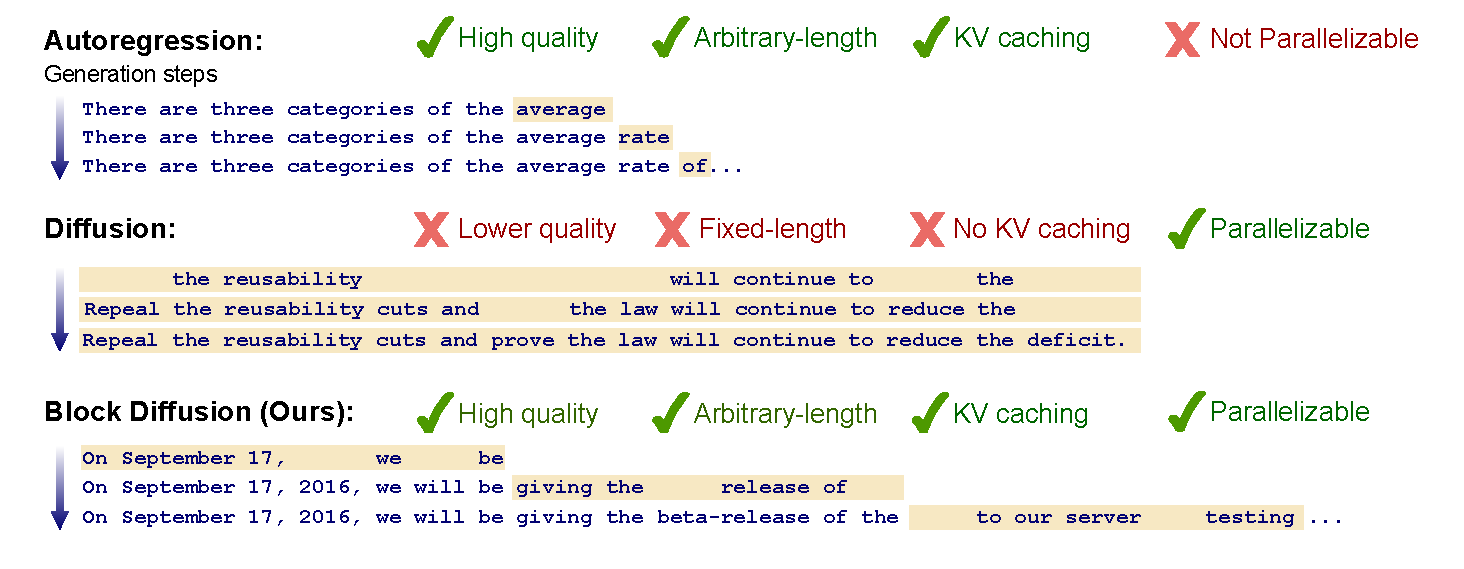
\includegraphics[width=1.1\textwidth]{figs/graphical_abstract.pdf}}
    \captionof{figure}{Block diffusion sequentially generates blocks of tokens by performing diffusion within each block and conditioning on previous blocks. By combining strength from autoregressive and diffusion models, block diffusion overcomes the limitations of both approaches by supporting variable-length, higher-quality generation and improving inference efficiency with KV caching and parallel sampling.}
    \label{figs/graphical-abstract}
    \vspace{-5pt}
\end{figure}

% \begin{figure}
%     \centering
%     \includegraphics[width=\linewidth]{figs/graphical_abstract_v2.pdf}
%     \caption{Block diffusion models blocks of tokens autoregressively and performs diffusion within each block. By combining strength from autoregressive and diffusion models, block diffusion overcomes the limitations of both approaches by supporting arbitrary-length, higher-quality generation and faster inference with KV-caching and parallel sampling.}
%     \label{fig:graphical-abstract}
% \end{figure}


We evaluate \algos{} on language modeling benchmarks, and demonstrate that they are able to generate sequences of arbitrary length, including lengths that exceed their training context. In addition, \algos{} achieve new state-of-the-art perplexities among discrete diffusion models. %, and make progress towards reducing the gap to autoregressive models. 
Compared to alternative semi-autoregressive formulations that perform Gaussian diffusion over embeddings \citep{han2022ssd,han2023ssd2}, our discrete approach features tractable likelihood estimates and yields samples with improved generative perplexity using an order of magnitude fewer generation steps.
% Semi-autoregressive diffusion models also feature natural speed advantages, as they can implement a forward pass over multiple tokens at inference time. We demonstrate that these models strike a natural trade-off between quality and speed that achieves points on the Pareto frontier that are not accessible with autoregressive models.
In summary, our work makes the following contributions:
\begin{itemize}
    % \item We introduce \algofull{} (\algos{}), which are autoregressive over blocks of tokens; conditionals over each block are based on discrete diffusion. Unlike prior diffusion language models, \algos{} support variable-length generation and KV-caching.
    \item We introduce block discrete diffusion language models, which are autoregressive over blocks of tokens; conditionals over each block are based on discrete diffusion. Unlike prior diffusion models, block diffusion supports variable-length generation and KV caching.
    \item  We introduce custom training algorithms for block diffusion models that enable efficiently leveraging the entire batch of tokens provided to the model.
    \item We identify gradient variance as a limiting factor of the performance of diffusion models, and we propose custom data-driven noise schedules that reduce gradient variance.
    \item Our results establish a new state-of-the-art perplexity for discrete diffusion and make progress toward closing the gap to autoregressive models.
\end{itemize}

%However, existing work has not shown its potential for likelihood modeling on standard benchmarks and have been limited to continuous diffusion models.
%We introduce a class of Precise Discrete Diffusion Language Models (\algos{}) that use a semi-autoregressive modeling framework and low-variance gradient estimators to close the likelihood gap with AR models.

%\algos{} achieve up to \TODO{...x} better perplexity relative to existing diffusion LMs and are within \TODO{...\%} of the autoregressive perplexity for block lengths \TODO{$L' \leq ...$}. Our analysis shows that the sample quality of \algos{} improves as $L' \rightarrow 1$ and the sample efficiency improves as $L' \rightarrow L$, which we analyze under unconditional generation and text summarization tasks.

%Our contributions are as follows:
%\begin{enumerate}
%\item We propose a semi-autoregressive (SAR) training recipe that strikes a balance between better likelihoods and faster inference by combining the strength of diffusion and autoregressive modeling
%\item We develop an efficient attention algorithm that predicts multiple tokens in parallel while supporting KV caching
%\item We introduce tunable noise schedules that further reduce the perplexity gap with autoregressive models by minimizing the variance of gradient updates during training
%\end{enumerate}

\section{Background: Language Modeling Paradigms}\label{sec:background}
\paragraph{Notation}
We consider scalar discrete random variables with $V$ categories as `one-hot' column vectors in the space $\mathcal{V} = \{\x \in \{0, 1\}^{V} : \sum_i \x_i = 1\}\subset \Delta^V$ for the simplex $\Delta^V$. Let the $V$-th category denote a special [MASK] token, where
$\m \in \mathcal{V}$ is its one-hot vector.
We define $\seqx$ as a sequence of $L$ tokens, where $\x^\ell \in \mathcal{V}$ for all tokens $\ell \in \{1, \ldots, L\},$ and use $\mathcal{V}^L$ to denote the set of all such sequences. Throughout the work, we simplify notation and refer to the token sequence as $\x$ and an individual token as $\x^\ell$. Finally, let $\cat(\cdot; p)$ be a categorical distribution with probability $p \in \Delta^V$. 
% \begin{enumerate}
%     \item Consider a sequence of $L$ tokens $\x = \left[ x^1, \dots, x^L \right]$ drawn from the data distribution $q(\mathbf{x})$. We aim to estimate the joint probability $p(\x)$. We compare two dominant language modeling frameworks: autoregressive and diffusion LMs.
% \end{enumerate}
\subsection{Autoregressive Models}
Consider a sequence of $L$ tokens $\x = \left[ \x^1, \dots, \x^L \right]$ drawn from the data distribution $q(\x)$. 
% Consider a sequence of $L$ tokens $\x = \left( x^1, \dots, x^L \right)$ drawn from the data distribution $q(\mathbf{x})$.  We aim to fit a model $p_\theta(\x)$ of $q$. 
% We compare two dominant language modeling frameworks: autoregressive and diffusion LMs.
Autoregressive (AR) models define a factorized distribution of the form
\begin{align}\label{eq:ar-nll}
    \log p_\theta(\x) = \sum_{\ell=1}^L \log p_\theta(\xl \mid \x^{<\ell}),
\end{align}
where each $p_\theta(\xl \mid \x^{<\ell})$ is parameterized directly with a neural network.
As a result, AR models may be trained efficiently via next token prediction. However, AR models take $L$ steps to generate $L$ tokens due to the sequential dependencies.

\subsection{Discrete Denoising Diffusion Probabilistic Models}
% \begin{enumerate}
%     \item Diffusion models learn $p(\mathbf{x})$ by iteratively undoing a forward corruption process $q(\mathbf{x})$. Whereas AR models optimize the true likelihood, diffusion models optimize a likelihood bound. 
%     \item Discrete diffusion models, such as D3PM \citep{austin2021structured}, define the diffusion process over discrete structures using a Markov forward process $q(\x_t | \x_{t-1}) = \cat( \x_t ; Q_t \x_{t-1})$. Masked diffusion language models are a class of discrete diffusion models that set the prior distribution to a "masked" state: $\boldsymbol{\pi} = \m$ \vkl{need less content on this than in MDLM, could even drop this bullet point} \TODO{introduce diffusion in the general D3PM formulation}
%     \item MDLM \citep{sahoo2023backpropagation} tightens the ELBO of this class of diffusion LMs and achieves state-of-the-art likelihoods among diffusion models  \TODO{use interpolating noise schedule from MDLM. Define $\alpha_t$ and other relevant notation. 1-2 sentences acknowledging the ELBO, call it $\mathcal{L}(\x, \theta)$}
    
% \end{enumerate}


% Diffusion models fit a model $p_\theta(\mathbf{x})$ to undo a forward corruption process $q$ \citep{sohl2015deep,ho2020denoising,sahoo2024diffusion}. This process starts with clean data $\x$ drawn from the data distribution $q(\x)$ and defines latent variables $\x_t$ for $t \in [0, 1]$  that represent progressively noisy versions of $\x$. In the discrete-time setting, 
% % the discrete denoising diffusion probabilistic modeling (D3PM) framework 
% the D3PM framework \citep{austin2021structured}
% defines $q$ to be a  Markov forward process $q(\x_t \mid \x_{t-1}) = \cat( \x_t ; Q_t \x_{t-1})$ where $Q_t \in \mathbb{R}^{V \times V}$  is the diffusion matrix. The $Q_t$ can encode masking, random token changes, related word substitutions, and more.
% % This process induces marginals
% % \begin{equation} \label{eq:d3pm_maginal}
% %     q(\x_t | \x) = \cat(\x_t ; \bar Q_t \x)  = \cat(\x_t ; Q_t \cdot Q_{t-1} \cdots Q_1 \x).
% % \end{equation}

% An ideal diffusion model $p_\theta$ is the reverse of the process $q$. The D3PM framework defines $p_\theta$ as 
% % the mean-parameterization is only insufficient for continuous distributions. we can use simple probability here because exact marginalization is tractable.
% %\begin{align}\label{eqn:diffusion}
% %    p_\theta(\x_s | \x_t) = q(\x_s | \x_t, \x_\theta(\x_t)) & \text{ where} & q(\x_s | \x_t, \x) = \cat(\x_s ; (Q_t \x \cdot \bar Q_{t-1} \x)/(\x_t^\top \bar Q_t \x))
% %\end{align}
% \begin{align}\label{eqn:diffusion}
%     p_\theta(\x_s \mid \x_t) = \sum_{\x}q(\x_s \mid \x_t, \x)p_\theta(\x\mid \x_t),
% \end{align}
% where the denoising base model $p_\theta(\x\mid\x_t)$ predicts clean tokens $\x$ given noised tokens $\x_t$.
% The marginalization is tractable due to the independent noising process over tokens in $q$, as well as the independence assumptions commonly made in the base model: the clean tokens are modeled independently as $\prod_i p(x^i\mid \x_t)$.
% %The posterior $q(\x_s | \x_t, \x)$ has an analytical form, but involves clean data $\x$, which is unavailable at generation time. Thus, D3PM introduces a model $\x_\theta(\x_t)$ of the clean data given noisy input $\x_t$.

% An ideal diffusion model $p_\theta$ is the reverse of the process $q$. The D3PM framework defines this model as $p_\theta(\x_s | \x_t)$ based on the posterior $q(\x_s | \x_t, \x) = \cat(\x_s ; (Q_t \x \cdot \bar Q_{t-1} \x)/(\x_t^\top \bar Q_t \x))$. Since the true data $\x$ is unavailable at generation time, D3PM introduces a model $\x_\theta(\x_t)$ of the clean data given noisy input $\x_t$ and defines $p_\theta(\x_s | \x_t) = q(\x_s | \x_t, \x_\theta(\x_t))$.

% % The parameterized reverse diffusion model $p_\theta$ over $\x$ and $\x_t$ is trained to maximize a variational lower bound on log-likelihood (ELBO).
% The diffusion model $p_\theta$ is trained using variational inference.
% Given a number of discretization steps $T,$ defining $s(j) = (j -1)/T$ and $ t(j) = j /T$, and using $\KL[\cdot]$ to denote the Kullback–Leibler divergence,
% % the Markov assumption on the forward and reverse processes allows us to express this ELBO as follows \citep{sohl2015deep}
% the Negative ELBO (NELBO) equals~\citep{sohl2015deep}:
% {\footnotesize
% \begin{align}\label{eqn:elbo}
%     % &\log p_\theta(\x) \geq \mathrm{ELBO}(p_\theta, q) \\ 
%     \mathcal{L}(\x) = \E_q\Bigg[- \log p_\theta(
%     \x | \x_{t(0)}) + \sum_{j=1}^T \KL[q(\x_{s(j)} | \x_{t(j)}, \x) \| p_\theta(\x_{s(j)} | \x_{t(j)})]
%     + \KL[q(\x_{t(T)} | \x) \| p_\theta(\x_{t(T)})] \Bigg]
% \end{align}
% }

% For brevity, we drop $j$ from $t(j)$ and $s(j)$ below; in general, $s$ will denote the time step before $t$.
% This formalism extends to continuous time via Markov chain (CTMC) theory, and admits score-based generalizations \citep{song2019generative, lou2024discrete, sun2022score} and simplifications \citep{sahoo2024simple, shi2024simplified, ou2025your} that tighten the ELBO and improve performance.
% % MDLM \citep{sahoo2024simple} tightens the ELBO of this class of diffusion LMs and achieves state-of-the-art likelihoods among diffusion models.

% NEW
Diffusion models fit a model $p_\theta(\mathbf{x})$ to reverse a forward corruption process $q$ \citep{sohl2015deep,ho2020denoising,sahoo2024diffusion}. This process starts with clean data $\mathbf{x}$ and defines latent variables $\mathbf{x}_t = \left[\mathbf{x}^1_t, \dots, \mathbf{x}^L_t\right]$ for $t \in [0, 1]$, which represent progressively noisier versions of $\mathbf{x}$. Given a discretization into $T$ steps, we define $s(j) = (j -1)/T$ and $t(j) = j /T$. For brevity, we drop $j$ from $t(j)$ and $s(j)$ below; in general, $s$ denotes the time step preceding $t$.

The D3PM framework \citep{austin2021structured} defines $q$ as a Markov forward process acting independently on each token $\mathbf{x}^\ell$:
$q(\mathbf{x}^\ell_{t} \mid \mathbf{x}^\ell_{s}) = \operatorname{Cat}(\mathbf{x}^\ell_t ; Q_t \mathbf{x}^\ell_{s})$
where $Q_t \in \mathbb{R}^{V \times V}$ is the diffusion matrix. The matrix $Q_t$ can model various transformations, including masking, random token changes, and related word substitutions. 

% The reverse posterior $q(\mathbf{x}^\ell_s \mid \mathbf{x}^\ell_t, \mathbf{x})$ is defined following \citet{austin2021structured} in \supp{supp:elbo}. Due to the unavailibility of $\x$ during inference, we approximate it using $\p: \mathcal{V} \times [0, 1] \to \Delta^K$ parameterized by a neural network with parameters $\theta$ as per the D3PM framework: 
An ideal diffusion model $\p$ is the reverse of the process $q$. The D3PM framework defines $\p$ as
\begin{align}\label{eqn:diffusion}
    p_\theta(\x_s \mid \x_t) = \prod_{\ell=1}^L p_\theta(\xl_s \mid \x_t) = \sum_{\x} \left[\prod_{\ell=1}^L q(\xl_s \mid \xl_t, \xl) p_\theta(\xl \mid \x_t)\right],
\end{align}
where the denoising base model $\p(\xl \mid \x_t)$ predicts clean token $\xl$ given the noisy sequence $\mathbf{x}_t$, and the reverse posterior $q(\mathbf{x}^\ell_s \mid \mathbf{x}^\ell_t, \mathbf{x})$ is defined following \citet{austin2021structured} in \supp{supp:elbo}. 
% The marginalization is tractable due to the independent noising process over tokens in $q$, as well as the independence assumptions commonly made in the base model: the clean tokens are modeled independently as $\prod_\ell p(\xl\mid \x_t)$.

The diffusion model $p_\theta$ is trained using variational inference. Let $\operatorname{KL}[\cdot]$ denote the Kullback-Leibler divergence. Then, the Negative ELBO (NELBO) is given by~\citep{sohl2015deep}:
{\footnotesize
\begin{align}\label{eqn:elbo}
    % &\log p_\theta(\x) \geq \mathrm{ELBO}(p_\theta, q) \\ 
    \mathcal{L}(\x; \theta) = \E_q\Bigg[- \log p_\theta(
    \x | \x_{t(1)}) + \sum_{j=1}^T \KL[q(\x_{s(j)} | \x_{t(j)}, \x) \| p_\theta(\x_{s(j)} | \x_{t(j)})]
    + \KL[q(\x_{t(T)} | \x) \| p_\theta(\x_{t(T)})] \Bigg]
\end{align}
}
This formalism extends to continuous time via Markov chain (CTMC) theory and admits score-based generalizations \citep{song2019generative, lou2024discrete, sun2022score}. Further simplifications \citep{sahoo2024simple, shi2024simplified, ou2025your} tighten the ELBO and enhance performance.

\section{Block Diffusion Language Modeling}
We explore a class of \algofull{} (\algos{}) that interpolate between autoregressive and diffusion models by defining an autoregressive distribution over blocks of tokens and performing diffusion within each block. We provide a block diffusion objective for maximum likelihood estimation and efficient training and sampling algorithms. We show that for a block size of one, the diffusion objective suffers from high variance despite being equivalent to the autoregressive likelihood in expectation. We identify high training variance as a limitation of diffusion models and propose data-driven noise schedules that reduce the variance of the gradient updates during training. 

% \paragraph{Notation}
% Consider a sequence of $L$ tokens $\x = \left[ x^1, \dots, x^L \right]$ drawn from the data distribution $q(\mathbf{x})$. We group tokens in $\x$ into $B$ blocks of length $L'$ with $B=B$ (we assume that $B$ is an integer). We denote each block $\x^{(b-1)L':bL'}$ from token at positions $(b-1)L'$ to $bL'$ for blocks $b \in \{ 1, \dots, B \}$ as $\x^b$ for simplicity.

\subsection{Block Diffusion Distributions and Model Architectures}\label{sec:sar-elbo}
We propose to combine the language modeling paradigms in Sec. \ref{sec:background} by autoregressively modeling blocks of tokens and performing diffusion within each block. 
% Let $L$ be the pre-training sequence length and $L'$ be the length of each SAR block, where $L' < L$. 
% Thus, log-likelihood factorizes over sequences of $L'$-length blocks as 
We group tokens in $\x$ into $B$ blocks of length $L'$ with $B=L/L'$ (we assume that $B$ is an integer). We denote each block $\x^{(b-1)L':bL'}$ from token at positions $(b-1)L'$ to $bL'$ for blocks $b \in \{ 1, \dots, B \}$ as $\x^b$ for simplicity. Our likelihood factorizes over blocks as
% where we have $B=L/L'$ blocks in the sequence. We denote each block $\x^{(b-1)L':bL'}$ from token at positions $(b-1)L'$ to $bL'$ for blocks $b \in \{ 1, \dots, B \}$ as $\x^b$ for simplicity:
\begin{align}\label{eqn:sar-ll}
     \log p_\theta(\x) &= \sum_{b = 1}^{B} \log p_\theta(\x^{b} \mid \x^{<b}),
\end{align}
and each $p_\theta(\x^b \mid \x^{<b})$ is modeled using discrete diffusion over a block of $L'$ tokens. 
% Specifically, a Markov forward noising process $q(\x_t^b|\x_s^b)$ is applied to $\x^b$; the reverse model $p_\theta(\x_s^b | \x_t^b, \x^{<b}) = q(\x_s^b | \x_t^b, \x^b_\theta(\x^b_t, \x^{<b}))$ is defined as in (\ref{eqn:diffusion}), but restricted to block $b$. 
Specifically, we define a reverse diffusion process as in (\ref{eqn:diffusion}), but restricted to block $b$:
%$p_\theta(\x_s^b | \x_t^b, \x^{<b}) = q(\x_s^b | \x_t^b, \x^b_\theta(\x^b_t, \x^{<b}))$
\begin{align}
    p_\theta(\x_s^b \mid \x_t^b, \x^{<b}) = \sum_{\x^b} q(\x_s^b \mid \x_t^b, \x^b)p_\theta(\x^b\mid \x^b_t,\x^{<b})
\end{align}
%Note that since each $p_\theta(\x^{b} \mid \x^{<b})$ is a distribution over $\x^{b} $ conditioned on $\x^{<b}$, the model $\x_\theta$ which denoises $\x^b_t$ is also conditioned on $\x^{<b}$.
We obtain a principled learning objective by applying the NELBO in (\ref{eqn:elbo}) to each term in (\ref{eqn:sar-ll}) to obtain
\begin{align}\label{eqn:sar-elbo}
    - \log p_\theta(\x) \leq \mathcal{L}_\text{BD}(\x; \theta) := \sum_{b=1}^{B} \mathcal{L}(\x^b, \x^{<b}; \theta),
\end{align}
where each $\mathcal{L}(\x^b, \x^{<b}; \theta)$ is an instance of (\ref{eqn:elbo}) applied to $\log p_\theta(\x^{b} \mid \x^{<b})$. Since the model is conditioned on $\x^{<b}$, we make the dependence on $\x^{<b}, \theta$ explicit in $\mathcal{L}$.
We denote the sum of these terms  $\mathcal{L}_\text{BD}(\x; \theta)$ (itself a valid NELBO).

% \marianne{We note that "block diffusion" modeling is synonymous with "}
% We adopt the simplified objective from \cite{sahoo2024simple} (the full derivation is provided in Suppl. \ref{supp:elbo}):
% \begin{align}\label{eqn:sar-elbo}
%     \mathcal{L}(\x, \theta) \geq \sum_{b=1}^{L/L'} \mathbb{E}_{t \sim [0, 1]} \mathbb{E}_{q} \frac{1}{1-\at} \log
%     \langle p_\theta(\x^b | \x_t^b, \x^{<b}), \x^b \rangle
% \end{align}
% The ELBO is tight for $B=1$ but becomes a looser approximation of the true log-likelihood for $B \rightarrow L$  (see Suppl. \ref{supp:sar-elbo-tightness}).

\paragraph{Model Architecture}
% ideally use f_\theta for the neural network
Crucially, we parameterize the $B$ base denoiser models $p_\theta(\x^b \mid \x^b_t, \x^{<b})$ using a single neural network $\x_\theta$. The neural network $\x_\theta$ outputs not only the probabilities $p_\theta(\x^b \mid \x_t^b, \x^{<b})$, but also computational artifacts for efficient training. This will enable us to compute the loss $\mathcal{L}_\text{BD}(\x; \theta)$ in parallel for all $B$ blocks in a memory-efficient manner.
Specifically, we parameterize $\x_\theta$ using a transformer \citep{vaswani2017attention} with a block-causal attention mask. The transformer $\x_\theta$ is applied to $L$ tokens, and tokens in block $b$ attend to tokens in blocks 1 to $b$. When $\x_\theta$ is trained, $\x^b_\theta(\x^b_t, \x^{<b})$ yields $L'$ predictions for denoised tokens in block $b$ based on noised $\x^b_t$ and clean $\x^{<b}$. % from previous blocks.

In autoregressive generation, it is normal to cache keys and values for previously generated tokens to avoid recomputing them at each step. Similarly, we use $\mathbf{K}^b, \mathbf{V}^b$ to denote the keys and values at block $b$, and we define $\x_\theta$ to support these as input and output. The full signature of $\x_\theta$ is
\begin{align}\label{eqn:model-kv}
    \x_\text{logits}^b, \mathbf{K}^b, \mathbf{V}^b \gets \x^b_\theta(\x^b_t, \mathbf{K}^{1:b-1}, \mathbf{V}^{1:b-1}) := \x^b_\theta(\x^b_t, \x^{<b}),
\end{align}
where $\x_\text{logits}^b$ are the predictions for the clean $\x^b$, and $\mathbf{K}^b, \mathbf{V}^b$ is the key-value cache in the forward pass of $\x_\theta$, and $\mathbf{K}^{1:b-1}, \mathbf{V}^{1:b-1}$ are keys and values cached on a forward pass of $\x_\theta$ over $\x^{<b}$ (hence the inputs $\x^{<b}$ and $\mathbf{K}^{1:b-1}, \mathbf{V}^{1:b-1}$ are equivalent). 

% In practice, we parameterize $p_\theta(\x^b |\x_t^b, \x^{<b})$ for blocks $\b \in 1, \dots, B$ in (\ref{eqn:sar-elbo}) using a transformer architecture. Our backbone takes as input a noised block $\x^b_{t_b} \sim q_{t_b}(\cdot|\x^b)$ and clean tokens in previous blocks $\x^{<b}$ to produce logits $\x_{\text{logit}} \gets \x_\theta^b(\x_{t_b}^b, \x^{<b})$.


\subsection{Efficient Training and Sampling Algorithms}\label{sec:eff-algs}

Ideally, we wish to compute the loss $\mathcal{L}_\text{BD}(\x; \theta)$ in one forward pass of $\x_\theta$. However, observe that denoising $\x_t^b$ requires a forward pass on this noisy input, while denoising the next blocks requires running $\x_\theta$ on the clean version $\x^b$. Thus every block has to go through the model at least twice.

\paragraph{Training}
Based on this observation, we propose a training algorithm with these minimal computational requirements
%
% However, this cannot be done in a normal forward pass through a classical transformer neural network since queries $Q^b$ at $\x_{t_b}^b$ must attend to keys and values $\mathbf{K}^{1:b\text{-}1}, \mathbf{V}^{1:b\text{-}1}$ of previous blocks $\x^{<b}$. 
% We propose to do so using a custom training algorithm 
(Alg.~\ref{alg:sar-train}). Specifically, we precompute keys and values $\mathbf{K}^{1:B}, \mathbf{V}^{1:B}$ for the full sequence $\x$ in a first forward pass $(\emptyset, \mathbf{K}^{1:B}, \mathbf{V}^{1:B}) \gets \x_\theta(\x)$.
We then compute denoised predictions for all blocks using $\x_\theta^b(\x_{t}^b,  \mathbf{K}^{1:b\text{-}1}, \mathbf{V}^{1:b\text{-}1})$. Each token passes through $\x_\theta$ twice.

\paragraph{Vectorized Training}

Naively, we would compute the logits by applying $\x_\theta^b(\x_{t}^b,  \mathbf{K}^{1:b\text{-}1}, \mathbf{V}^{1:b\text{-}1})$ in a loop $B$ times. We propose a vectorized implementation that computes $\mathcal{L}_\text{BD}(\x; \theta)$ in one forward pass on the concatenation $\x_\text{noisy} \oplus \x$ of clean data $\x$ with  noisy data $\x_\text{noisy} = \x^1_{t_1} \oplus \dots \oplus \x^B_{t_B}$ obtained by applying a noise level $t_b$ to each block $\x^b$. We design an attention mask for $\x_\text{noisy} \oplus \x$ such that noisy tokens attend to other noisy tokens in their block and to all clean tokens in preceding blocks
(see Suppl. \ref{suppl:masks}).  Our method keeps the overhead of training \algos{} tractable and combines with pretraining to further reduce costs.
% In practice, this procedure is about 50\% slower than diffusion training. 

% As a result, we efficiently model the conditional likelihoods between blocks relative to a naive implementation that requires $B$ forward passes for each conditional term. We may do so using two forward passes (one for pre-computing keys and values $\mathbf{K}^{1:B}, \mathbf{V}^{1:B}$ and the second for computing logits $\x_{\text{logit}}$), or through a single forward pass on $\x_t \oplus \x$ using a custom mask to mimic the proposed attention pattern (more details in Suppl. \ref{suppl:masks}).


\paragraph{Sampling} We sample one block at a time, conditioned on previously sampled blocks (Alg \ref{alg:sar-inference}). We may use any sampling procedure $ \textsc{Sample}(\x_\theta^b, \mathbf{K}^{1:b\text{-}1},\mathbf{V}^{1:b\text{-}1})$ to sample from the conditional distribution $p_\theta(\x_{s}^b | \x_{t}^b, \x^{<b})$, where the context conditioning is generated using cross-attention with pre-computed keys and values $\mathbf{K}^{1:b-1}, \mathbf{V}^{1:b-1}$. Similar to AR models, caching the keys and values saves computation instead of recalculating them when sampling a new block.

Notably, our block diffusion decoding algorithm enables us to sample sequences of arbitrary length, whereas diffusion models are restricted to fixed-length generation. Further, our sampler admits parallel generation within each block, whereas AR samplers are constrained to generate token-by-token.

% \begin{multicols}{2}
%     \begin{algorithm}[H]
%     \caption{BAR training}
%     \label{alg:sar-train}
%     \begin{algorithmic}
%     \State \textbf{Input:} $\x_0 \sim q_0$, $L$ seq. len., $B$ \# of blocks
%     \State $\M \gets \Mask(L, B)$ (Suppl. \ref{suppl:masks})
%     \Repeat
%         \State Sample $t_1, \dots, t_B \sim \mathcal{U}(0, 1)$
%         \State $\x_t \sim q_t(\x_0)$
%         \State $\x_{\text{full}} \gets \x_{t} \oplus \x_0$
%         \State $\x_{\text{full}} = h_\theta(\x_{\text{full}}; \M)$
%         \State Take gradient step on $\nabla_\theta \mathcal{L}_{BAR}(\x_{\text{full}})$
        
%     \Until{converged}
%     \end{algorithmic}
%     \end{algorithm}
    
%     \columnbreak
    
%     \begin{algorithm}[H]
%     \caption{BAR Sampling}
%     \label{alg:sar-inference}
%     \begin{algorithmic}
%     \State \textbf{Input:} $p_{\text{limit}}$, $T$ diffusion steps, $L$ seq.len, $B$ \# of blocks
%     \State \textbf{Output:} $\tilde{\x}^0$ \vkl{can probably reduce \# of lines, e.g., drop this one}
    
%     \State $\tilde{\x}^0 \gets \emptyset$ 
%     \State $K, V \gets \emptyset$  \Comment{KV cache}
%     \State $\M \gets \textsc{BlockCausalMask}(L, B)$
    
%     \For{$b = 1$ to $B$}
%         \State $\x_T \sim p_{\text{limit}}$ \vkl{what's p limit?}
%         \State $\tilde{\x}_{0} \gets \tilde{\x}_0 \oplus \x_T$ \vkl{why do we need this?}

%         \For{$t = T$ to $1$}
%             \State $\tilde{\x}_0, K, V \gets h_\theta(\tilde{\x}_0, K, V, \M)$ \vkl{what is $h$? this doesn't sound right: the $t$ doesn't appear inside the loop, and also this doesn't look like an actual MDLM sampler}
%         \EndFor
%     \EndFor
    
% \State \Return $\tilde{\x}_0$
% \end{algorithmic}
% \end{algorithm}
% \end{multicols}
    

\begin{multicols}{2}
    \begin{algorithm}[H]
    \caption{Block Diffusion Training}
    \label{alg:sar-train}
    \begin{algorithmic}
    \State \textbf{Input:} datapoint $\x$, \# of blocks $B$, forward noise process $q_t(\cdot|\x)$, model $\x_\theta$, loss $\mathcal{L}_{\text{BD}}$
    \Repeat
        \State Sample $t_1, \dots, t_B \sim \mathcal{U}[0, 1]$
        % \State Sample $\x_{t_1}^1, \dots, \x^B_{t_B} \sim q_{t_1}, \dots, q_{t_B}$
        \State $\forall b \in \{1,...,B\}:$ $\x_{t_b}^b \sim q_{t_b}(\cdot|\x^b)$
        \State $\emptyset, \mathbf{K}^{1:B}, \mathbf{V}^{1:B} \gets \x_\theta(\x)$ \Comment{KV cache}
        \State $\forall b \text{: } \x_\text{logit}^b, \emptyset, \emptyset \gets \x_\theta^b(\x_{t_b}^b,  \mathbf{K}^{1:b\text{-}1}, \mathbf{V}^{1:b\text{-}1})$ 
        \State Let $\x_\text{logit} \gets \x_\text{logit}^1 \oplus \dots \oplus \x^B_\text{logit}$
        \State Take gradient step on $\nabla_\theta \mathcal{L}_{\text{BD}}(\x_{\text{logit}}; \theta)$
        
    \Until{converged}
    \end{algorithmic}
    \end{algorithm}
    
    \columnbreak
    
    \begin{algorithm}[H]
    \caption{Block Diffusion Sampling}
    \label{alg:sar-inference}
    \begin{algorithmic}
    \State \textbf{Input:} \# blocks $B$, model $\x_\theta$, diffusion sampling algorithm \textsc{Sample}
    \vspace{3pt}
    
    \State $\x, \mathbf{K},\mathbf{V} \gets \emptyset$ \Comment{output \& KV cache}
    \vspace{3pt}
    \For{$b = 1$ to $B$}
        % \State $\x_0^b, \mathbf{K}^b,\mathbf{V}^b \gets \textsc{Sample}(\x_\theta^b, \mathbf{K}^{:b\text{-}1},\mathbf{V}^{:b\text{-}1})$
        \State $\x^b \gets \textsc{Sample}(\x_\theta^b, \mathbf{K}^{1:b\text{-}1},\mathbf{V}^{1:b\text{-}1})$
        \State $\emptyset, \mathbf{K}^{b}, \mathbf{V}^{b} \gets \x_\theta^b(\x^b)$
        \State $\x \gets \x^{1:b-1} \oplus \x^b $
        \State $(\mathbf{K}, \mathbf{V}) \gets (\mathbf{K}^{1:b-1} \oplus \mathbf{K}^b, \mathbf{V}^{1:b-1} \oplus \mathbf{V}^b) $
        % \State $\mathbf{V} \gets \mathbf{V}^{1:b-1} \oplus \mathbf{V}^b $
    \EndFor
    
\State \Return $\x$
\end{algorithmic}
\end{algorithm}
\end{multicols}
    


\section{Understanding Likelihood Gaps Between Diffusion \& AR Models}

% \subsection{\algofull{} (\algos{})}
\subsection{Masked \algos{}}

The most effective diffusion language models leverage a masking noise process \citep{austin2021structured,lou2024discrete,sahoo2024simple}, where tokens are gradually replaced with a special mask token. Here, we introduce masked \algos{}, a special class of block diffusion models based on the masked diffusion language modeling framework \citep{sahoo2024simple, shi2024simplified, ou2025your}.

More formally, we adopt a per-token noise process $q(\xl_t| \xl) = \cat(\xl_t; \at \xl + (1 - \at) \m)$ for tokens $\ell \in \{1, \dots, L\}$
where $\m$ is a one-hot encoding of the mask token, and $\alpha_t \in [0, 1]$
is a strictly decreasing function in $t$, with $\alpha_{0} = 1$ and $\alpha_{1} = 0$. We employ the linear schedule where the probability of masking a token at time $t$ is $1-\alpha_t$.
We adopt the simplified objective from \cite{sahoo2024simple, shi2024simplified, ou2025your} (the full derivation is provided in Suppl. \ref{supp:elbo}):
\begin{align}\label{eqn:sar-elbo-exp}
    - \log p_\theta(\x) \leq \mathcal{L}_\text{BD}(\x; \theta) :=  \sum_{b=1}^{B} \mathbb{E}_{t \sim [0, 1]} \mathbb{E}_{q} \frac{\at'}{1-\at} \log p_\theta(\x^b | \x_{t}^b, \x^{<b})
\end{align}
\noindent where $\at'$ is the instantaneous rate of change of $\at$ under the continuous-time extension of (\ref{eqn:elbo}) that takes $T \rightarrow \infty$. The NELBO is tight for $L'=1$ but becomes a looser approximation of the true negative log-likelihood for $L' \rightarrow L$  (see Suppl. \ref{supp:sar-elbo-tightness}).

\subsection{Case Study: Single Token Generation}
\begin{wraptable}{r}{5cm}
    \small
  \vspace{-15pt}
  \caption{Test perplexities for single-token generation (PPL; $\downarrow$) across 16B tokens on LM1B.}
  \label{tab:bs1-var}
  \centering
  \begin{tabular}{lll}
    \toprule
    & PPL ($\downarrow$)  \\
    \midrule
    AR  & \textbf{22.88} \\
    \hspace{1em} + random batch size & 24.37 \\
    \midrule
    \algo{} $L'=1$ & $\leq$ 25.56\\
    \hspace{1em} + tuned schedule & \textbf{22.88} \\
    \bottomrule
  \end{tabular}
  \vspace{-10px}
\end{wraptable}
Our block diffusion parameterization (\ref{eqn:sar-elbo-exp}) is equivalent in expectation to the autoregressive NLL (\ref{eq:ar-nll}) in the limiting case where $L'=1$ (see Suppl. \ref{supp:sar-block1-nll}). Surprisingly, we find a two point perplexity gap between our block diffusion model for $L'=1$ and AR when training both models on the LM1B dataset.


Although the objectives are equivalent in expectation, we show that the remaining perplexity gap is a result of high training variance. Whereas AR is trained using the cross-entropy of $L$ tokens, our block diffusion model for $L'=1$ only computes the cross-entropy for masked tokens $\xl_t = \m \; \forall \ell \in \{ 1, \dots L \}$ so that $\mathbb{E}_{t \sim \mathcal{U}[0,1]} q(\xl_t = \m | \xl) = 0.5$. Thus, training on the diffusion objective involves estimating loss gradients with 2x fewer tokens and is responsible for higher training variance compared to AR.

To close the likelihood gap, we train a \algo{} for $L'=1$ by designing the forward process to fully mask tokens, i.e. $q(\xl_t = \m | \xl) =1$. Under this schedule, the diffusion objective becomes \textit{equivalent} to the AR objective (Suppl. \ref{supp:sar-block1-nll}). In Table \ref{tab:bs1-var}, we show that training under the block diffusion objective yields the same perplexity as AR training. Empirically, we see that this reduces the variance of the training loss in Figure \ref{figs/bs-1}. We verify  that tuning the noise schedule reduces the variance of the objective by measuring $\text{Var}_{\x, t} \left[ \mathcal{L}_{\text{BD}} (\x; \theta)\right]$ after training on 328M tokens: while training on the NELBO results in a variance of 1.52, training under full masking reduces the variance to 0.11.
\begin{figure}
\centering
    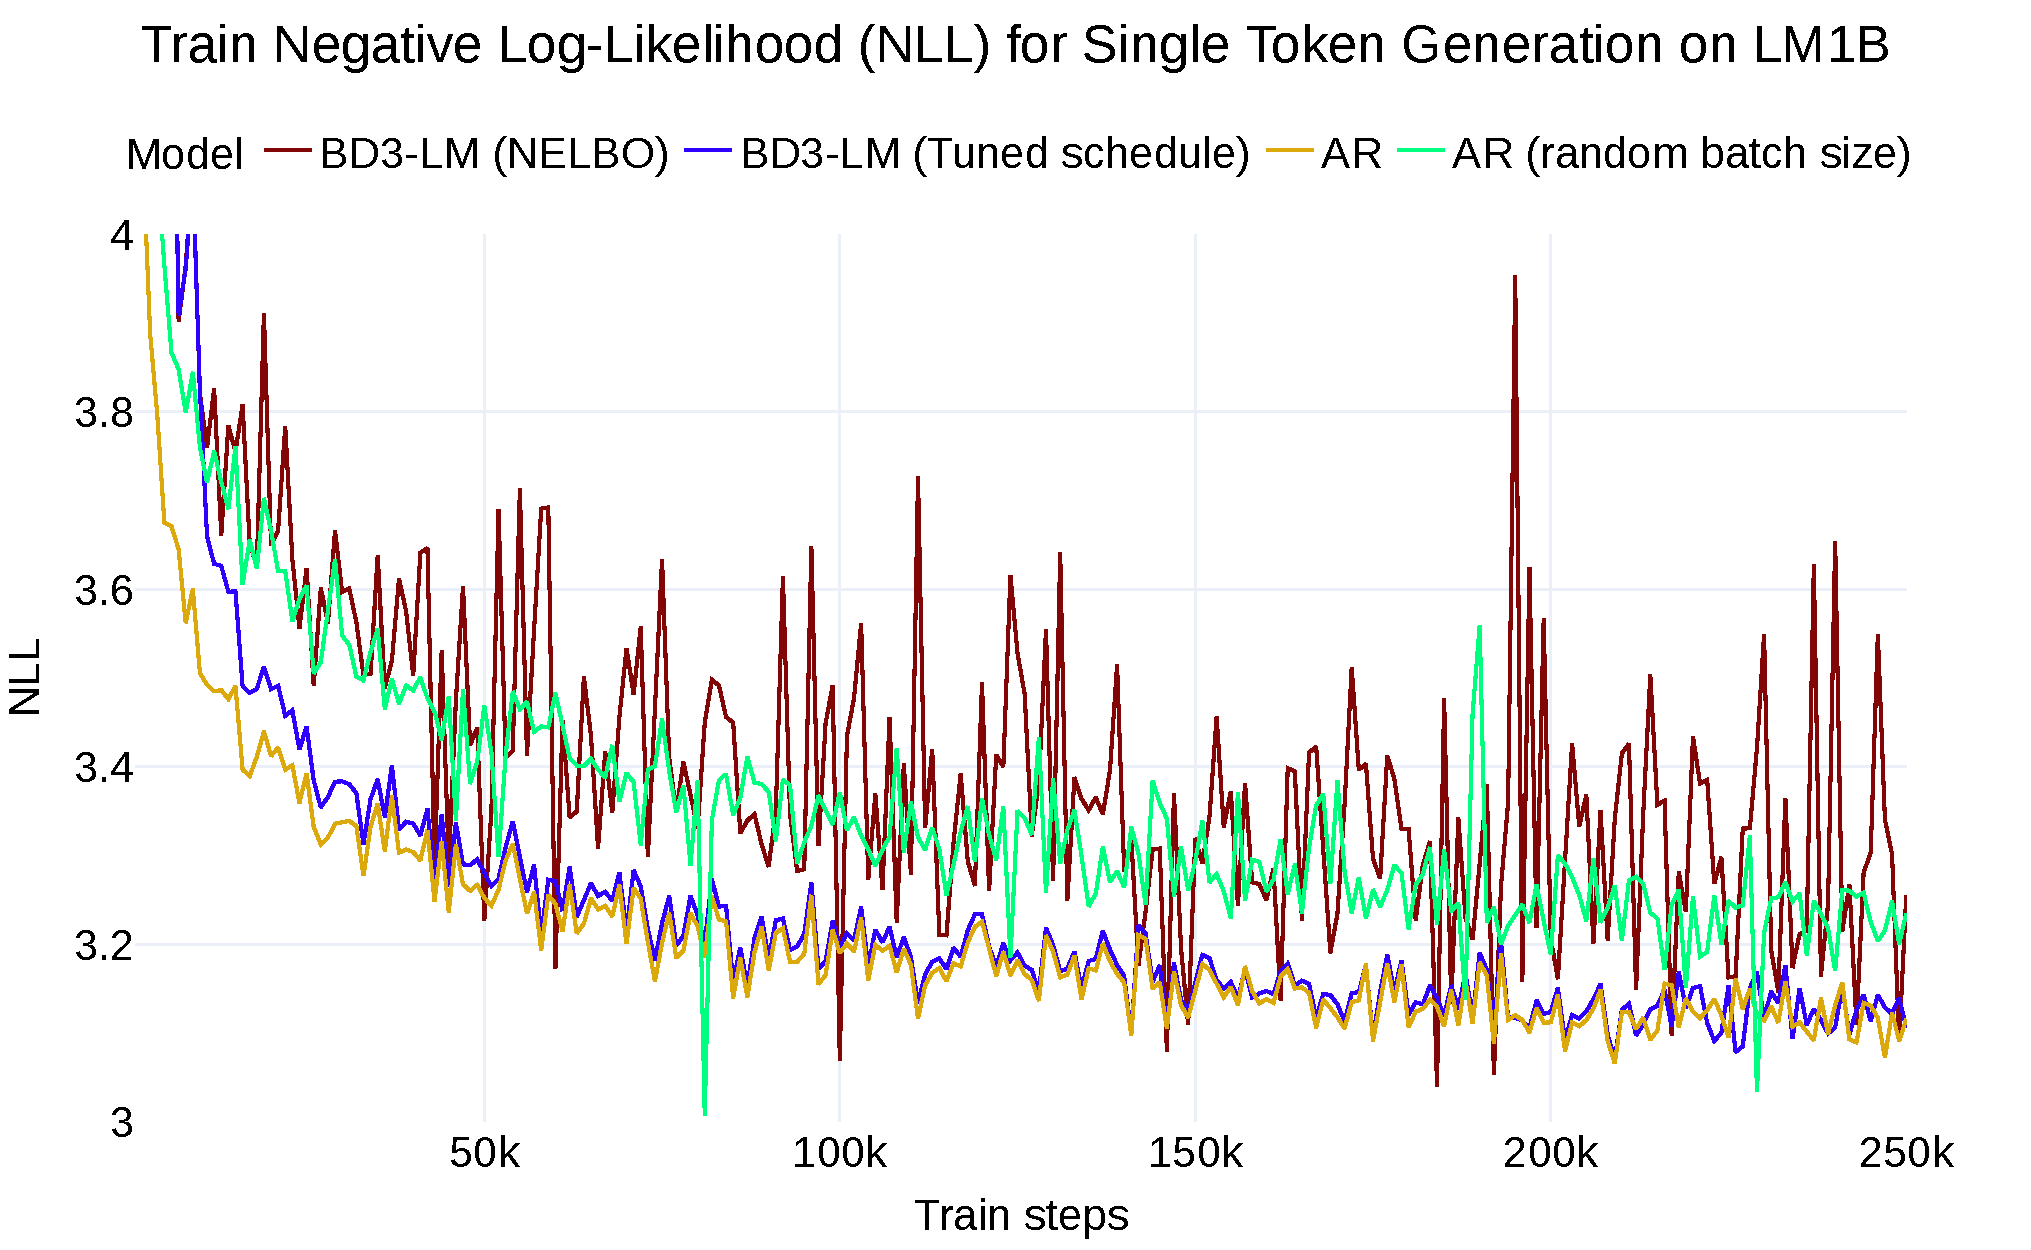
\includegraphics[width=0.75\textwidth]{figs/bs1.pdf}
    \captionof{figure}{Train NLLs for modeling the per-token likelihood on LM1B. Models are trained on 16B tokens. Training under the discrete diffusion NELBO, where half of the tokens in a batch are masked on average, has similar training variance to an AR model with a random batch size.}
    \label{figs/bs-1}
\end{figure}


\subsection{Diffusion Gap from High Variance Training}
Next, we formally describe the issue of gradient variance in training diffusion models. Given our empirical observations for single-token generation, we propose an estimator for gradient variance that we use to minimize the variance of diffusion model training for $L' \geq 1$. While the NELBO is invariant to the choice of noise schedule (Suppl. \ref{supp:elbo}), this invariance does not hold for our Monte Carlo estimator of the loss used during training. %for sampling $\x \sim q_0, t \sim \mathcal{U}[0, 1]$, $\x_t \sim q_t(\x)$. 
As a result, the variance of the estimator and its gradients are dependent on the schedule. First, we express the estimator of the NELBO %$l_\theta (\x)$
with a batch size $K$.
We denote a batch of sequences as $\mathbf{X} = \left[\x^{(1)}, \x^{(2)}, \ldots, \x^{(K)}\right]$, with each $\x^{(k)}\overset{\text{iid}}\sim q(\x)$. We obtain the batch NELBO estimator below, where $t(k, b)$ is sampled in sequence $k$ and block $b$:
\begin{align}
\mathcal{L}_\text{BD}(\mathbf{X}; \theta)
:= l(\mathbf{X}; \theta)
= \frac{1}{K} \sum_{k=1}^K \sum_{b=1}^B  \frac{\alpha_{t(k, b)}'}{1-\alpha_{t(k,b)}}
\log p_\theta \left(
    \x^{(k),b} \mid \x_{t(k,b)}^{(k),b}, \x^{(k), <b}
\right)
\end{align}
% We derive a Monte Carlo estimator of the diffusion ELBO over batch size $K$ and $B$ blocks:
% \begin{align}\label{eq:estimator}
%    \mathcal{L}_{[0, 1]}(\theta ; \mathbf{X}) &= \mathbb{E}_{\x \sim q_0} \sum_{b=1}^{B}  \mathbb{E}_{t \sim [0, 1]} \mathbb{E}_{q} \frac{1}{1 - \at} \log \langle p_\theta(\x_t^b | \x^{<b}), \x^b \rangle \\
%    &\approx \frac{1}{K} \sum_{k=1}^K \sum_{b=1}^B  \frac{1}{1-\alpha_{t_b}} \log \langle p_\theta(\x_{t_b}^{k, b} | \x^{k, <b}), \x^{k, b} \rangle 
% \end{align}
% \vkl{may want to briefly define the new variables}



% \begin{align}
%     \nabla_\theta \mathbb{E}_{\x \sim q(\x)} [\mathcal{L}_\text{MDLM}(\x)] &\approx  \hat{g}_{[0,1]} = \frac{1}{K} \sum_{k=1}^K \sum_{b=1}^B \frac{\alpha'_t}{1-\alpha_{t_{k,b}}}  \nabla_\theta \log p_\theta(\x^{k, b} \mid \x_{t_{k,b}}^{k, b}, x^{k, <b})  
% \end{align}
% \noindent where under the linear schedule $\at = 1 - t$, $\at'$ is constant across $t \in [0, 1]$.

% We now analyze the variance of the gradient estimator. For simplicity we define the gradient of the Monte Carlo loss estimate as $l_\theta$:
% % \begin{align}
% %     f_\theta (\x_t) = \nabla_\theta  \log \langle p_\theta(\x_t^b | \x^{<b}), \x^b \rangle \quad \text{and} \quad \bar{f}_\theta = \frac{1}{K} \sum_{k=1}^K\sum_{b=1}^B\sum_{i=1}^M  \frac{\alpha_t'}{1-\alpha_{t_i}} \nabla_\theta \log \langle p_\theta(\x_{t_i}^{b} | \x^{<b}), \x^{b} \rangle
% % \end{align}


The variance of the gradient estimator over $M$ batches for each batch $\mathbf{X}^m \; \forall m \in \{ 1, \dots, M\}$ is:
 \begin{align}\label{eq:grad-var-estimator}
     \text{Var}_{\mathbf{X}, t}\left[
    \nabla_\theta l (\mathbf{X}; \theta) \right] 
&\approx  \frac{1}{M-1} \sum_{m=1}^M \left\lVert 
    \nabla_\theta l (\mathbf{X}^m; \theta) - \frac{1}{M} \sum_{m=1}^M \nabla_\theta l(\mathbf{X}^m; \theta)
\right\rVert^2_2
\end{align}
 % \vkl{small aesthetic question: you introduce $1/(1-\alpha_t)$ in (9) for one term and in (10) for the other term, is that intentional?}


%, \x_t \sim q_t(\x), \x \sim q_0$. 

%\vkl{the superscript notation is overloaded and in one formula we use k to denote a datapoints in a batch, and in the other one we use k (or $k_m$) to denote the batch itself}

% \subsubsection{Pitfalls of gradient estimation under sampling uniform mask rates}

% \vkl{I don't think we need this section anymore?}

% We observe empirically that the gradient estimator $\nabla_\theta g (\x)$ under uniformly sampling mask rates $1 - \alpha_t \sim \mathcal{U}[0, 1]$ suffers from high variance. As we saw in the case of modeling a single token, we observed high variance training that contributed to a 2 point perplexity gap on LM1B and high-variance gradient estimates.

% In Table \ref{tab:lm1b_vars}, we observe that training using uniformly sampled mask rates results in higher-variance estimates of the NLL compared to training on a subset of masking rates.

\section{Low-Variance Noise Schedules for \algos{}}
 % We use the above observations to derive improved, low-variance gradient estimators for \algos{} that control the noise schedule.

 \subsection{Intuition: Avoid Extreme Mask Rates}
We aim to identify schedules that minimize the variance of the gradient estimator and make training most efficient. 
%
In a masked setting, we want to mask random numbers of tokens, so that the model learns to undo varying levels of noise, which is important during sampling.
However, if we mask very few tokens, reconstructing them is easy and does not provide useful learning signal. If we mask everything, the optimal reconstruction are the marginals of each token in the data distribution, which is easy to learn, and again is not useful. These extreme masking rates lead to poor high-variance gradients: we want to learn how to clip them via a simple and effective new class of schedules.
% However, the precise optimal sampling distribution depends on the size of the block: we saw that for small blocks, we may want to mask everything, while larger blocks would benefit from smaller rate
% We attribute high-variance training to sampling extreme masking rates. Intuitively, if the mask rate $1-\alpha_t$ is too low, most tokens are unmasked the denoising task is too easy and the gradient is not useful for training. Similarly, if the masking rate is too high, then the Bayes optimal solution is to predict the marginals of the data distribution. \TODO{might be a bit too hand-wavey}

% Furthermore, our empirical analysis on the variance of our proposed gradient estimator demonstrate that sampling lighter mask rates results in high-magnitude gradients. However, for larger block sizes $L' \geq 8$, there exists a threshold where masking that is too heavy will result in low-quality logits from limited context.

% \vkl{I think we can expand more on this intuition. I think the idea is that if the mask is too high, the problem is too easy (you just predict the marginals of the data) and the gradient is not useful; if the mask \% is too low, then it's also too easy (nothing is masked) and the gradient is not useful}

\subsection{Clipped Schedules for Low-Variance Gradients}
% We reduce the variance of the gradient estimator by avoiding sampling $t$ that induce high variance in our gradient estimator.

We propose a class of ``clipped'' noise schedules that sample mask rates $1-\at \sim \mathcal{U}[\beta, \omega]$ for $0 \leq \beta, \omega \leq 1$. We argue that from the perspective of deriving Monte Carlo gradient estimates, these schedules are equivalent to a continuous schedule where the mask probability is approximately 0 before the specified range such that $1-\alpha_{<\beta} \approx \epsilon$ and approximately 1 after the specified range $1-\alpha_{>\omega} \approx 1-\epsilon$. Consequently, $\at'$ is linear within the range: $\at' \approx 1 / (\beta - \omega)$.
% % \vkl{this bracket notation is a bit confusing}. 
% We derive the Monte Carlo estimators of the diffusion ELBO under such clipped schedules:
% \begin{align}\label{eq:clipped-estimator}
%    \mathcal{L}_{[\beta, \omega]}(\theta ; \mathbf{X}) &\approx \frac{1}{K} \sum_{k=1}^K \sum_{b=1}^B \sum_{i=1}^M  \frac{\beta - \omega}{1-\alpha_{t_i}} \log \langle p_\theta(\x_{t_i}^b | \x^{<b}_k), \x^b_k \rangle 
% \end{align}

% \begin{align}
%     f_\theta (\x_t) = \nabla_\theta \log \langle p_\theta(\x_t^b | \x^{<b}), \x^b \rangle \quad \text{and} \quad \bar{f}_\theta = \frac{1}{K} \sum_{k=1}^K\sum_{b=1}^B \sum_{i=1}^M  \frac{\beta - \omega}{1-\alpha_{t_i}} \nabla_\theta \log \langle p_\theta(\x_{t_i} | \x^{<b}_k), \x^{b}_k \rangle
% \end{align}
% \vkl{above $f$ is not a function of $\omega, \beta$} \vkl{also many comments from previous section apply here}We propose a new gradient estimator for these schedules, $\hat{g}_{[\beta, \omega]}$. We derive the variance of the gradient estimator of our linear schedule $\hat{g}_{[\beta, \omega]}$ as where $t \sim \mathcal{U}[\beta, \omega], \x_t \sim q_t(\x), \x \sim q_0$. We propose the estimator :

%  \begin{align}\label{eq:grad-var-estimator}
%       \text{Var}_{\x, t}\left[ \nabla_\theta g \right] &=  \frac{1}{M-1} \sum_{m=1}^M \left\lVert \nabla_\theta l_\theta (\x^{m}) - \frac{1}{M} \sum_{m=1}^M \nabla_\theta l_\theta(\x^m) \right\rVert^2_2
% \end{align}

% We show that there exists $\beta, \omega$ that improves the variance of the gradient estimate: $\text{Var}_{\x, t} \left[\hat{g}_{[\beta,\omega]}\right] < \text{Var}_{\x, t} \left[\hat{g}_{[0, 1]}\right]$.
% \TODO{need a proof, can put the full proof in the appendix. just need to show that increasing the bounds increases the variance}

\subsection{Data-Driven Clipped Schedules Across Block Sizes}\label{sec:data-driven-schedules}
As the optimal mask rates may differ depending on the block size $L'$, we adaptively learn the schedule during training. While \cite{kingma2021variational} perform variance minimization by isolating a variance term using their squared diffusion loss, this strategy is not directly applicable to our variance estimator in Equation \ref{eq:grad-var-estimator} since we seek to reduce variance across random batches in addition to random $t_b$.

Instead, we optimize parameters $\beta, \omega$ to directly minimize training variance. To limit the computational burden of the optimization, we use the variance of the estimator of the diffusion ELBO as a proxy for the gradient estimator to optimize $\beta, \omega$: $\min_{\beta, \omega} \text{Var}_{\mathbf{X}, t} \left[ \mathcal{L}(\mathbf{X}; \theta, \beta, \omega) \right]$. We perform a grid search at regular intervals during training to find the optimal $\beta, \omega$ (experimental details in Sec. \ref{sec:experiments}).

In Table \ref{tab:lm1b_vars}, we show that variance of the diffusion NELBO is correlated with test perplexity. Under a range of ``clipped'' noise rate distributions, we find that there exists a unique distribution for each block size $L' \in \{4, 16, 128\}$ that minimizes both the variance of the NELBO and the test perplexity.



\begin{table*}[ht]
    \small
  \caption{Perplexities (PPLs; $\downarrow$) and variances of the NELBO $\text{Var}_{\mathbf{X}, t}\left[ \mathcal{L}_\text{BD}(\mathbf{X}; \theta)  \right]$ (Var. NELBO; $\downarrow$). Models are trained on LM1B using a linear schedule for 65B tokens, then finetuned for 10B tokens.}
  \label{tab:lm1b_vars}
  \centering
  \setlength{\tabcolsep}{6pt} % Adjust horizontal padding
  \renewcommand{\arraystretch}{1.1} % Adjust vertical space between rows
  \begin{tabular}{ccccccccc}
    \toprule
     & \multicolumn{2}{c}{$\mathcal{U}[0, .5]$} & \multicolumn{2}{c}{$\mathcal{U}[.3, .8]$} & \multicolumn{2}{c}{$\mathcal{U}[.5, 1]$} & \multicolumn{2}{c}{$\mathcal{U}[0, 1]$}  \\
    \cmidrule(lr){2-3} \cmidrule(lr){4-5} \cmidrule(lr){6-7} \cmidrule(lr){8-9}
    $L'$     & PPL & Var. NELBO & PPL & Var. NELBO & PPL & Var. NELBO & PPL & Var. NELBO \\
    \midrule
    128  & \textbf{31.72}  & \textbf{1.03} & 31.78   &  1.35  &  31.92 & 1.83 &  31.78 & 3.80  \\
    16 &  31.27 & 7.90 & \textbf{31.19} & \textbf{3.62} &  31.29  & 3.63 &     31.33 & 7.39 \\
    4   &  29.23 & 32.68 & 29.37  & 10.39 & \textbf{29.16}   & \textbf{8.28} & 29.23  &  23.65 \\
    \bottomrule
  \end{tabular}
\end{table*}


\begin{wraptable}{r}{0.45\textwidth}
  \vspace{-20pt}
  \small
  \caption{Test perplexities (PPL; $\downarrow$) of models trained for 65B tokens on LM1B. Best diffusion value is bolded.}
  \label{tab:lm1b-ppl}
  \centering
  \vspace{-10pt}
  \setlength{\tabcolsep}{2pt} % Reduce column padding
  \begin{tabular}{lc}
    \toprule
      & PPL ($\downarrow$) \\
    \midrule
    \multicolumn{2}{l}{\textbf{Autoregressive}} \\
    Transformer-X Base{~\citep{dai2019transformer}}  &  23.5 \\
    $\text{Transformer}$~\citep{sahoo2024simple}  & 22.83 \\
    \midrule
    \multicolumn{2}{l}{\textbf{Diffusion}} \\
    D3PM (absorb)~\citep{austin2021structured}  & $\leq$ 82.34  \\
    SEDD ~\citep{lou2024discrete}  & $\leq$ 32.68   \\
    MDLM ~\citep{sahoo2024simple}  & $\leq$ 31.78\\
    \midrule
    \multicolumn{2}{l}{\textbf{Block diffusion (Ours)}} \\
    \algos{} $L'=16$   & $\leq$ 30.60 \\ 
    \hspace{4.1em} $L'=8$   & $\leq$ 29.83\\
    \hspace{4.1em} $L'=4$  & $\leq$ \textbf{28.23}  \\
    \bottomrule
  \end{tabular}
  \vspace{-20pt}
\end{wraptable}

\section{Experiments}\label{sec:experiments}

We evaluate \algos{} across standard language modeling benchmarks and demonstrate their ability to generate arbitrary-length sequences unconditionally. We pre-train a base \algo{} using the maximum block size $L'=L$ for 850K gradient steps and fine-tune under varying $L'$ for 150K gradient steps on the One Billion Words dataset (LM1B; \citet{chelba2014billion}) and OpenWebText (OWT; \citet{Gokaslan2019OpenWeb}). Details on training and inference are provided in Suppl \ref{suppl:details}.

To reduce the variance of training on the diffusion NELBO, we adaptively learn the range of masking rates by optimizing parameters $\beta, \omega$ as described in Section \ref{sec:data-driven-schedules}. In practice, we do so using a grid search during every validation epoch (after $\sim$5K gradient updates) to identify $\beta, \omega$: $\min_{\beta, \omega} \text{Var}_{\mathbf{X}, t} \left[ \mathcal{L}(\mathbf{X}; \theta, \beta, \omega) \right]$. During evaluation, we report likelihood under uniformly sampled mask rates (\ref{eqn:sar-elbo-exp}) as in \citet{austin2021structured, sahoo2024simple}.

\begin{wraptable}{r}{0.4\textwidth}
\vspace{-10pt}
\small
\centering
    \caption{Test perplexities (PPL; $\downarrow$) on \owt{} for models trained for 524B tokens. Best diffusion value is bolded.}\label{owt-ppl}
  \begin{tabular}{ll}
    \toprule
    & PPL ($\downarrow$) \\
    \midrule
    AR~\citep{sahoo2024simple} & 17.54 \\
    \midrule
    SEDD~\citep{lou2024discrete} & $\leq$ 24.10 \\
    MDLM~\citep{sahoo2024simple} & $\leq$ 22.98 \\
    \midrule
    \algos{} $L'=16$ & $\leq$ 22.27 \\
    \hspace{4.3em}$L'=8$ & $\leq$ 21.68  \\
    \hspace{4.3em}$L'=4$ & $\leq$ \textbf{20.73} \\
    \bottomrule
  \end{tabular}
\vspace{-15pt}
\end{wraptable}

% \vkl{Consider having a section where you just look at the ability to generate arbitrary length text. You want to argue that previous discrete diffusion models (at least SEDD out of the box) cannot generate full-length documents that are longer than the length of the output context chosen at training time. This can be purely qualitative. For example, you can generate documents on OWT and report the length distribution of training data, SEDD-generated data (which would be clipped after 1024), and your data (which should go beyond 1024). If you could show an improvement over MDLM with SAR sampling, that would be awesome, but if not, we can shove it under the rug. We might also be able to add more quantitative experiments.}


\subsection{Likelihood Evaluation}
On LM1B, \algos{} outperform all prior diffusion methods in Table \ref{tab:lm1b-ppl}. Compared to MDLM~\citep{sahoo2024simple}, \algos{} achieve up to 13\% improvement in perplexity.  We observe a similar trend on OpenWebText in Table \ref{owt-ppl}.


We also evaluate the ability of \algos{} to generalize to unseen datasets in a zero-shot setting, following the benchmark from \citet{radford2019language}. We evaluate the likelihood of models trained with OWT on datasets Penn Tree Bank (PTB; \citep{marcus1993building}), Wikitext \citep{merity2016pointer}, LM1B, Lambada \citep{paperno-EtAl:2016:P16-1}, AG News \citep{Zhang2015CharacterlevelCN}, and Scientific Papers (Pubmed and Arxiv subsets; \citep{Cohan_2018}). In Table \ref{zeroshot-ppl}, \algo{} achieves the best zero-shot perplexity on Pubmed, surpassing AR, and the best perplexity among diffusion models on Wikitext, LM1B, and AG News.
% \begin{table*}[ht]
% \small
% \caption{Zero-shot validation perplexities ($\downarrow$) of models trained for 524B tokens on \owt{}.
% All perplexities for diffusion models are upper bounds.
% }
% \small
% \label{zeroshot-ppl}
% \centering
% \begin{tabular}{lccccccccc}
% \toprule
% & PTB & Wikitext & LM1B & Lambada  & AG News & Pubmed & Arxiv\\
% \midrule
% AR &\underline{81.07}& \underline{25.32}& \underline{51.14} & 52.13 & \underline{52.11} & 48.59 & 41.22\\
% \midrule
% SEDD  & 96.33 & 35.98 & 68.14& 48.93 & 67.82 & 45.39 & 40.03\\
% MDLM  &\textbf{90.96}& 33.22& 64.94& \underline{\textbf{48.29}} & 62.78 & 43.13 & \underline{\textbf{37.89}}\\
% \algo{} $L'=4$ & 96.81 & \textbf{31.31} & \textbf{60.88} & 50.03 & \textbf{61.67} & \underline{\textbf{42.52}} & 39.20\\

% \bottomrule
% \end{tabular}
% % \vspace{-4.5pt}
% \end{table*}All perplexities for diffusion models are upper bounds.


\begin{table*}[ht]
\small
\caption{Zero-shot validation perplexities ($\downarrow$) of models trained for 524B tokens on \owt{}.
All perplexities for diffusion models are upper bounds.
}
\small
\label{zeroshot-ppl}
\centering
\begin{tabular}{lccccccccc}
\toprule
& PTB & Wikitext & LM1B & Lambada  & AG News & Pubmed & Arxiv\\
\midrule
AR &\textbf{81.07}& \textbf{25.32}& \textbf{51.14} & 52.13 & \textbf{52.11} & 48.59 & 41.22\\
\midrule
SEDD  & 96.33 & 35.98 & 68.14& 48.93 & 67.82 & 45.39 & 40.03\\
MDLM  &90.96& 33.22& 64.94& \textbf{48.29} & 62.78 & 43.13 & \textbf{37.89}\\
\algo{} $L'=4$ & 96.81 & 31.31 & 60.88 & 50.03 & 61.67 & \textbf{42.52} & 39.20\\

\bottomrule
\end{tabular}
% \vspace{-4.5pt}
\end{table*}

\subsection{Sample Quality and Variable-Length Sequence Generation}\label{subsec:samples}

\begin{wraptable}{r}{0.38\textwidth}
    \small
    \vspace{-10pt}
  \caption{Generation length statistics from sampling 500 documents from models trained on OWT.}
  \label{tab:owt-gen-lens}
  \centering
    \setlength{\tabcolsep}{2pt} % Reduce column padding

  \begin{tabular}{lcc}
  
    \toprule
    & Median  & Max \\
    & \# tokens  & \# tokens \\

    \midrule
    OWT train set  & 717 & 131K\\
    AR  & 4008 & 131K \\
    \midrule
    SEDD & 1021 & 1024 \\
    \algo{} $L'=16$ & 798 & 9982\\
    \bottomrule
  \end{tabular}
  \vspace{-5pt}
\end{wraptable}

% \begin{wraptable}{r}{0.57\textwidth}
%     \small
%   \vspace{-11pt}
%   \setlength{\tabcolsep}{2.0pt} % Reduce column padding
%   \renewcommand{\arraystretch}{0.9} % Reduce row height
%   \caption{Generative perplexity (Gen. PPL; $\downarrow$) of \TODO{200} samples of length $L=1024, 2048$. All models are trained on OWT and use nucleus sampling. Experimental details are in Suppl. \ref{suppl:eval-details}.}
%   \label{tab:gen_ppl_2048}
%   \centering
%     \begin{tabular}{lcccc}
%       \toprule
%       & \multicolumn{2}{c}{$L=1024$} & \multicolumn{2}{c}{$L=2048$} \\
%       \cmidrule(lr){2-3} \cmidrule(lr){4-5}
%       Model & Gen. PPL & NFEs & Gen. PPL & NFEs \\
%       \midrule
%       AR & 14.5 & 1K & 13.1 & 2K \\
%       \midrule 
%       \multicolumn{5}{l}{\textbf{Diffusion}} \\
%       SEDD & 53.2 & 1K & -- & -- \\
%       MDLM & 46.3 & 1K & 38.1 & 2K \\
%       \midrule
%       \multicolumn{5}{l}{\textbf{Block Diffusion}} \\
%       SSD-LM $L'=25$ & 36.9 & 40K & 35.2 & 80K  \\
%       & 325.8 & 1K & 278.1 & 2K  \\
%       \algos{} $L'=16$ & 37.4 & 1K & 36.5 & 2K \\
%       \hspace{4.1em} $L'=8$ & 34.9 & 1K & 35.5 & 2K \\
%       \hspace{4.1em} $L'=4$ & \textbf{28.5} & 1K & \textbf{27.9} & 2K \\
%       \bottomrule
%     \end{tabular}
%   \vspace{-8pt}
% \end{wraptable}

% We assess the capacity of \algos{} to generate high-quality, variable-length samples. 

One key drawback of many existing diffusion language models (e.g,. \citet{austin2021structured,lou2024discrete}) is that they cannot generate full-length sequences that are longer than the length of the output context chosen at training time. The OWT dataset is useful for examining this limitation, as it contains many documents that are longer than the training context length of 1024 tokens. 

% We assess the capacity of \algos{} to generate high-quality, variable-length samples by examining generation length statistics as well as generative perplexity under GPT2-Large for varying decoding lengths (experimental details provided in Suppl. \ref{suppl:eval-details}).


We record generation length statistics of 500 variable-length samples in Table \ref{tab:owt-gen-lens}. We continue sampling tokens until an end-of-sequence token [EOS] is generated or sample quality significantly degrades (as measured by sample entropy). \algos{} generate sequences up to $\approx$10$\times$ longer than those of SEDD \citep{lou2024discrete}, which is restricted to the training context size.

We also examine the sample quality of \algos{} through quantitative and qualitative analyses. In Table \ref{tab:gen_ppl_2048}, we generate sequences of lengths $L=1024, 2048$ and measure their generative perplexity under GPT2-Large. To sample $L=2048$ tokens from MDLM, we use their block-wise decoding technique (which does not feature block diffusion training as in \algos{}).

We also compare to SSD-LM \citep{han2022ssd}, an alternative block diffusion formulation. Unlike our discrete diffusion framework, SSD-LM uses Gaussian diffusion and does not support likelihood estimation. Further, \algo{} adopts an efficient sampler from masked diffusion, where the number of generation steps (NFEs) is upper-bounded by $L$ since tokens are never remasked~\citep{sahoo2024simple, ou2025your}. For SSD-LM, we compare sample quality using $T=1$K diffusion steps per block, matching their experimental setting (yielding $\geq$40K NFEs), and $T=25$ where NFEs are comparable across methods.


\begin{table}[ht!]
    \small
  \caption{Generative perplexity (Gen. PPL; $\downarrow$) and number of function evaluations (NFEs; $\downarrow$) of 300 samples of lengths $L=1024, 2048$. All models are trained on OWT. AR, SEDD, MDLM, \algos{} use 110M parameters and are trained on 524B tokens, while SSD-LM uses 400M parameters and is pre-trained on 122B tokens. Best diffusion value is bolded. We provide further details in Suppl. \ref{suppl:eval-details}.}
  \label{tab:gen_ppl_2048}
  \centering
    \begin{tabular}{lcccc}
      \toprule
      & \multicolumn{2}{c}{$L=1024$} & \multicolumn{2}{c}{$L=2048$} \\
      \cmidrule(lr){2-3} \cmidrule(lr){4-5}
      Model & Gen. PPL & NFEs & Gen. PPL & NFEs \\
      \midrule
      AR & 14.1 & 1K & 13.2 & 2K \\
      \midrule 
      \multicolumn{5}{l}{\textbf{Diffusion}} \\
      SEDD & 52.0 & 1K & -- & -- \\
      MDLM & 46.8 & 1K & 41.3 & 2K \\
      \midrule
      \multicolumn{5}{l}{\textbf{Block Diffusion}} \\
      SSD-LM $L'=25$ & 37.2 & 40K & 35.3 & 80K  \\
      & 281.3 & 1K & 281.9 & 2K  \\
      \algos{} $L'=16$ & 33.4 & 1K & 31.5 & 2K \\
      \hspace{4.1em} $L'=8$ & 30.4 & 1K & 28.2 & 2K \\
      \hspace{4.1em} $L'=4$ & \textbf{25.7} & 1K & \textbf{23.6} & 2K \\
      \bottomrule
    \end{tabular}
    % \vspace{-10pt}
\end{table}


% \algos{} also enjoy efficiency improvements over AR models by using fewer functional evaluations (NFEs), whereas AR generation is fixed to $L$ NFEs. We evaluate our proposed BAR decoding algorithm (Alg. \ref{alg:sar-inference}) in unconditional generation generate 50 sequences of lengths $L = 1024$ using \algos{}. We show that BAR approaches support generating sequences of arbitrary length, overcoming a key limitation of sampling with diffusion models. In generating 1024 tokens (Table \ref{tab:gen_ppl_2048}), \algo{} may achieve better quality than SSD-LM while using much fewer NFEs.
% \begin{table*}[ht]
\algos{} achieve the best generative perplexities compared to previous diffusion methods. Relative to SSD-LM, our discrete approach yields samples with improved generative perplexity using an order of magnitude fewer generation steps. We also qualitatively examine samples taken from \algo{} and baselines (AR, MDLM) trained on the OWT dataset; we report samples in Suppl. \ref{suppl:summaries}. We observe that \algo{} samples have higher coherence than MDLM samples and approach the quality of AR.


\subsection{Ablations}\label{sec:ablation}
We assess the impact of the design choices in our proposed block diffusion recipes, namely 1) selection of the noise schedule and 2) the efficiency improvement of the proposed training algorithm relative to a naive implementation.

\subsubsection*{Selecting Noise Schedules to Reduce Training Variance}

% Our class of data-driven "clipped" noise schedules are the most effective in reducing the perplexity gap compared to linear, cosine, and logarithmic schedules. We find that "clipping" the masking rates during training is the most effective for reducing the variance of the training objective, which correlates with the perplexity.  In Table \ref{tab:var_ns_training}, we train \algos{} under a variety of different schedules for $L'=4, 16$ and show their impact on test perplexity on LM1B. The ideal "clipped" masking rates, which are optimized during training, are specific to the block size and further motivate our optimization.

Compared to the linear schedule used in \citet{lou2024discrete, sahoo2024simple}, training under ``clipped'' noise schedules is the most effective for reducing the training variance which correlates with test perplexity. In Table \ref{tab:var_ns_training}, the ideal ``clipped'' masking rates, which are optimized during training, are specific to the block size and further motivate our optimization. 

\begin{wraptable}{r}{0.43\textwidth}
  \vspace{-13pt}
  \small
  \caption{Effect of the noise schedule on likelihood estimation. We finetune \algos{} on 3B tokens from LM1B and evaluate on a linear schedule. For clipped schedules, we compare optimal clipping for \(L' = 4, 16\).}
  \vspace{-8pt}
  \label{tab:var_ns_training}
  \centering
  \begin{tabular}{lcc}
    \toprule
    Noise schedule & PPL & Var. NELBO \\
    \midrule
    \textbf{L' = 4} &&\\
    Clipped &&\\
    \quad \(\mathcal{U}[0.45, 0.95]\) & \textbf{29.21} & \textbf{6.24} \\
    \quad \(\mathcal{U}[0.3, 0.8]\) & 29.38 & 10.33 \\
    Linear \(\mathcal{U}[0,1]\) & 30.18 & 23.45 \\
    Logarithmic & 30.36 & 23.53 \\
    Square root & 31.41 & 26.43 \\
    \midrule
    \textbf{L' = 16} &&\\
    Clipped &&\\
    \quad \(\mathcal{U}[0.45, 0.95]\) & 31.42 & 3.60 \\
    \quad \(\mathcal{U}[0.3, 0.8]\) & \textbf{31.12} & \textbf{3.58} \\
    Linear \(\mathcal{U}[0,1]\) & 31.72 & 7.62 \\
    Square & 31.43 & 13.03 \\
    Cosine & 31.41 & 13.00 \\
    \bottomrule
  \end{tabular}
  \vspace{-40pt}
\end{wraptable}

Relative to other standard noise schedules \citep{chang2022maskgit}, ``clipped'' masking achieves the best performance. As heavier masking is effective for the smaller block size $L'=4$, we compare with logarithmic and square root schedules that also encourage heavy masking. As lighter masking is optimal for $L'=16$, we compare with square and cosine schedules.



\subsubsection*{Efficiency of Training Algorithm}
In the \algo{} training algorithm (Sec. \ref{sec:eff-algs}), we compute $\x_{\text{logit}}$ using two options. We may perform two forward passes through the network (precomputing keys and values for the full sequence $\x$, then computing denoised predictions), or combine these passes by concatenating the two inputs into the same attention kernel.



We find that a single forward pass is more efficient as we reduce memory bandwidth bottlenecks by leveraging efficient attention kernels~\citep{dao2022flashattention, dong2024flex}, see Suppl. \ref{suppl:flex-attention-kernels}. Instead of paying the cost of two passes through the network, we only pay the cost of a more expensive attention operation. Our vectorized approach has 20-25\% speed-up during training relative to performing two forward passes.


\section{Discussion and Prior Work}

% \vkl{TODO: re-phrase the comparison to D3PM, add section on SSD-LM, maybe find one more comparison? also need to edit conclusion}

\paragraph{Comparison to D3PM}
Block diffusion builds off D3PM \citep{austin2021structured} and applies it to each autoregressive conditional. We improve over D3PM in three ways: (1) we extend D3PM beyond fixed sequence lengths; (2) we study the perplexity gap of D3PM and AR models, identify gradient variance as a contributor, and design variance-minimizing schedules; (3) we improve over the perplexity of D3PM models. 
% Note that (2) is applicable to vanilla D3PM, not just our block-wise extension. 
Our work applies to extensions of D3PM \citep{he2022diffusionbert,lou2024discrete} including ones in continuous time \citep{campbell2022continuous,sun2022score}.
% While (1) involves modifying D3PM to make it block-wise, (2) is applicable to vanilla D3PM. 


\paragraph{Comparison to MDLM}
\algos{} further make use of the perplexity-enhancing improvements in MDLM \citep{sahoo2024simple,shi2024simplified,ou2025your}. We also build upon MDLM: (1) while \citet{sahoo2024simple} point out that their NELBO is invariant to the noise schedule, we show that the noise schedule has a significant effect on gradient variance; (2) we push the state-of-the-art in perplexity beyond MDLM. Note that our perplexity improvements stem not only from block diffusion, but also from optimized schedules, and could enhance standard MDLM and D3PM models.

\paragraph{Comparison to Gaussian Diffusion} Alternatively, one may perform diffusion over continuous embeddings of discrete tokens \citep{li2022diffusion, dieleman2022continuous, chen2022analog}. This allows using algorithms for continuous data \citep{song2020denoising,ho2022classifier}, but yields worse perplexity \citep{graves2023bayesian,gulrajani2024plaid}.

\paragraph{Comparison to Semi-Autoregressive Diffusion}
\citet{han2022ssd,han2023ssd2} introduced a block formulation of Gaussian diffusion. \algos{} instead extend \citet{austin2021structured}, and feature: (1) tractable likelihood estimates for principled evaluation; (2) faster generation, as our number of model calls is bounded by the number of generated tokens, while SSD-LM performs orders of magnitude more calls; (3) improved sample quality. AR-Diffusion \citep{wu2023ardiffusion} extends SSD-LM with a left-to-right noise schedule; \citet{chen2025diffusion, ye2024diffusion} apply to decision traces and videos; \citet{hao2024training,kong2025scalable} extend to latent reasoning. PARD \citep{zhao2024pard} applies discrete block diffusion to graphs. In contrast, we (1) interpolate between AR/diffusion performance; (2) support KV caching; (3) perform attention within noised blocks, whereas PARD injects new empty blocks.

% diffuser
Autoregressive diffusion models \citep{hoogeboom2021argmax,hoogeboom2021autoregressive} extend any-order AR models (AO-ARMs; \citet{uria2014deep}) to support parallel sampling. \citet{zheng2024masked} prove equivalence between MDLM and AO-ARM training.
Further extensions of ARMs that compete with diffusion include iterative editing \citep{gu2019levenshtein}, parallel and speculative decoding \citep{gu2017non,santilli2023accelerating,cai2024medusa,gloeckle2024better}, consistency training \citep{kou2024cllms}, guidance \citep{sanchez2023stay}, and cross-modal extensions \citep{liu2023visual,tian2025visual}.

\paragraph{Limitations}

Training \algos{} is more expensive than regular diffusion training. We propose a vectorized algorithm that keeps training speed within <2x of diffusion training speed; in our experiments, we also pre-train with a standard diffusion loss to further reduce the speed gap. Additionally, \algos{} generate blocks sequentially, and hence may face the same speed and controllability constraints as AR especially when blocks are small. Their optimal block size is task specific (e.g., larger for greater control).
% and optimal blocks for speed depend on the parallelization capabilities of inferencing hardware (e.g,. FLOPS vs.~memory throughput) and serving batch size.
\algos{} are subject to inherent limitations of generative models, including hallucinations \citep{achiam2023gpt}, copyright infringement \citep{gokaslan2024commoncanvas}, controllability \citep{schiff2024discreteguidance,wang2023infodiff} and harmful outputs \citep{bai2022constitutional}. % which require further research.

\section{Conclusion}
This work explores block diffusion and is motivated by two problems with existing discrete diffusion: the need to generate arbitrary-length sequences and the perplexity gap to autoregressive models. We introduce \algos{}, which represent a block-wise extension of the D3PM framework \citep{austin2021structured}, and leverage a specialized training algorithm and custom noise schedules that further improve performance. We observe that in addition to being able to generate long-form documents, these models also improve perplexity, setting a new state-of-the-art among discrete diffusion models.
% These models can generate factually inaccurate or misleading information, commonly referred to as hallucinations, particularly when extrapolating beyond their training data. Additionally, they may produce outputs that inadvertently replicate biases present in the training corpus. Copyright concerns also arise, as models trained on large-scale datasets may generate text resembling protected content, raising questions about data provenance and responsible deployment. Addressing these challenges remains crucial for ensuring the reliability and ethical use of generative models.

\subsubsection*{Acknowledgments and Disclosure of Funding}
This work was partially funded by the National Science Foundation under awards DGE-1922551,
CAREER awards 2046760 and 2145577,  and by the National Institute of Health under award MIRA
R35GM151243. Marianne Arriola is supported by a NSF Graduate Research Fellowship under award DGE-2139899 and a Hopper-Dean/Bowers CIS Deans Excellence Fellowship. We thank Databricks MosaicML for providing access to computational resources.


\bibliography{iclr2025_conference}
\bibliographystyle{iclr2025_conference}

\newpage

\appendix
\setcounter{tocdepth}{2}
\tableofcontents
\allowdisplaybreaks


\section{Block Diffusion NELBO}\label{suppl:diffusion-nelbo}
Below, we provide the Negative ELBO (NELBO) for the block diffusion parameterization. Recall that the sequence $\x^{1:L} = \left[ \x^1, \dots, \x^L \right]$ is factorized over $B$ blocks, which we refer to as $\x$ for simplicity, drawn from the data distribution $q(\mathbf{x})$. Specifically, we will factorize the likelihood over $B$ blocks of length $L'$, then perform diffusion in each block over $T$ discretization steps. Let $\KL[\cdot]$ to denote the Kullback-Leibler divergence, $t, s$ be shorthand for $t(i) = i / T$ and $s(i) = (i - 1)/T$ $\forall i \in [1, T]$. We derive the NELBO as follows:
\begin{align}\label{eq:nelbo-bd}
    - \log \p(\x) &= - \sum_{b = 1}^{B} \log \p(\x^{b} | \x^{<b}) \nonumber \\
    &=  - \sum_{b = 1}^{B} \log \mathbb{E}_{q} \frac{\p(\x^{b}_{t(1):t(T)} | \x^{<b})}{q(\x^{b}_{t(1):t(T)} | \x^{b})} \nonumber \\
    &=  - \sum_{b = 1}^{B} \log \mathbb{E}_{q}   \frac{ \p(\x^{b}_{t(T)}| \x^{<b}) \prod_{i=1}^T \p(\x^{b}_{s(i)}| \x^{b}_{t(i)}, \x^{<b})}{ \prod_{i=1}^T q(\x^{b}_{t(i)} | \x^{b}_{s(i)})} \nonumber \\
    &\leq \sum_{b = 1}^{B} \bigg[ \underbrace{- \mathbb{E}_{q} \log \p(\x^{b} | \x_{t = \frac{1}{T}}^{b}, \x^{<b})}_{\mathcal{L}_{\text{recons}}} \notag \\
    & \hspace{4em} + \underbrace{\mathbb{E}_{t \in \left\{ \frac{2}{T}, \dots, \frac{T - 1}{T}, 1 \right\}}  \mathbb{E}_{q} T  
      \text{D}_{KL}\left( q(\x^{b}_{s} | \x^{b}_{t}, \x^{b}) \parallel 
      \p(\x^{b}_{s}| \x^{b}_{t}, \x^{<b})\right)}_{\mathcal{L}_{\text{diffusion}}} \notag \\
    & \hspace{4em} + \underbrace{\text{D}_{KL} \left( q(\x^{b}_{t=1} | \x^{b}) \parallel \p(\x^{b}_{t=1}) \right)}_{\mathcal{L}_{\text{prior}}} \bigg ] 
\end{align}
% \noindent For simplicity, we will denote $s = (t - 1)/ T$. 


\section{Masked \algos{}}

We explore a specific class of block diffusion models that builds upon the masked diffusion language modeling framework. In particular, we focus on masking diffusion processes introduced by \citet{austin2021structured} and derive a simplified NELBO under this framework as proposed by~\citet{sahoo2024simple, shi2024simplified, ou2025your}.

First, we define the diffusion matrix $Q_t$ for states $i \in \{1, \dots, V\}$. Consider the noise schedule function $\alpha_t \in [0, 1]$, which is a strictly decreasing function in $t$ satisfying $\alpha_{0} = 1$ and $\alpha_{1} = 0$. Denote the mask index as $m=V$. The diffusion matrix is defined by~\citet{austin2021structured} as:
\begin{align}
    [Q_t]_{ij} =
    \begin{cases}
    1 & \text{if } i = j = m \\
    \at & \text{if } i = j \neq m \\
    1-\at & \text{if } j = m, i \neq m
    \end{cases}
\end{align}

The diffusion matrix for the forward marginal $\Qts$ is:
\begin{align}
    [Q_{t|s}]_{ij} =
    \begin{cases}
    1 & \text{if } i = j = m \\
    \ats & \text{if } i = j \neq m \\
    1-\ats & \text{if } j = m, i \neq m
    \end{cases}
\end{align}
\noindent where $\ats = \at / \as$.


\subsection{Forward Process}

Under the D3PM framework \citep{austin2021structured}, the forward noise process applied independently for each token $\ell \in \{1, \dots L\}$ is defined using diffusion matrices $Q_t \in \mathbb{R}^{V \times V}$ as
\begin{align}
q(\xl_t | \xl) = \text{Cat} \left( \xl_t; \overline{Q}_t \xl \right), \quad \text{with} \quad \overline{Q}_{t(i)} = Q_{t(1)} Q_{t(2)} \dots Q_{t(i)}
\end{align}


\subsection{Reverse Process}

Let $\Qts$ denote the diffusion matrix for the forward marginal. We obtain the reverse posterior $q(\xl_s \mid \xl_t, \xl)$ using the diffusion matrices:
\begin{align}
q(\xl_{s} | \xl_t, \xl) = \frac{q(\xl_t | \xl_{s}, \xl) q(\xl_{s} | \xl)}{q(\xl_t | \xl)} = \text{Cat} \left( \xl_{s}; \frac{Q_{t|s} \xl_t \odot Q_s^\top \xl}{{(\xl_t)}^\top  Q_t^\top \xl} \right)
\end{align}
\noindent where $\odot$ denotes the Hadmard product between two vectors.



\subsection{Simplified NELBO for Masked Diffusion Processes} \label{supp:elbo}


Following \cite{sahoo2024simple, shi2024simplified, ou2025your}, we simplify the NELBO in the case of masked diffusion processes. Below, we provide the outline of the NELBO derivation; see the full derivation in \cite{sahoo2024simple, shi2024simplified, ou2025your}.

% We will first focus on the simplifying the diffusion loss term $\mathbb{E}_{t \in \{ 2, \dots T \}}  \mathbb{E}_{q} T  \text{D}_{KL}\left( q(\x^{b}_{s} |, \x^{b}_{t}, \x^{b}_{0}) \parallel \p(\x^{b}_{t-1}| \x^{b}_{t}, \x^{<b})\right)$. 

We will first focus on simplifying the diffusion loss term $\mathcal{L}_\text{diffusion}$ in Eq. \ref{eq:nelbo-bd}. We employ the SUBS-parameterization proposed in~\citet{sahoo2024diffusion} which simplifies the denoising model $\p$ for masked diffusion. In particular, we enforce the following constraints on the design of $\p$ by leveraging the fact that there only exists two possible states in the diffusion process $\xl_t \in \{ \xl, \m \} \; \forall \ell \in \{1, \dots, L\}$. 
\begin{enumerate}
    \item \textbf{Zero Masking Probabilities}. We set $p_\theta(\xl = \m | \xl_t) = 0$ (as the clean sequence $\x$ doesn't contain masks).
    \item \textbf{Carry-Over Unmasking}. The true posterior for the case where $\xl_t \neq \m$ is $q(\xl_s = \xl_t | \xl_t \neq \m) = 1$ (if a token is unmasked in the reverse process, it is never remasked). Thus, we simplify the denoising model by setting $p_\theta (\xl_s = \xl_t | \xl_t \neq \m) = 1$.
\end{enumerate}
As a result, we will only approximate the posterior $\p(\xl_s = \xl | \xl_t = \m)$. Let $\x^{b, \ell}$ denote a token in the $\ell$-th position in block $b \in \{1, \dots, B\}$. The diffusion loss term becomes:
\begin{align}
    % &/ \mathcal{L}_{\text{diffusion}} \nonumber \\
    % & = \sum_{b = 1}^{B} \mathbb{E}_{t} \mathbb{E}_{\x} T \left[  q(\x_s^b | \x^b_t, \x^b) \log \frac{q(\x_s^b | \x_t^b, \x^b)}{\p(\x_s^b = \x^b | \x_t^b=\m, \x^{<b})} \right] \nonumber \\
    % & = \sum_{b = 1}^{B} \mathbb{E}_{t} \mathbb{E}_{\x} T\left[ \left[\prod_{\ell = 1}^{L'}  q(\xlb_s | \xlb_t, \xlb)\right] \log  \frac{\prod_{\ell = 1}^{L'} q(\xlb_s | \xlb_t, \xl)}{\prod_{\ell = 1}^{L'} \p(\xlb_s  | \xlb_t=\m, \x^{<b})} \right] \nonumber \\
    % & = \sum_{b = 1}^{B} \mathbb{E}_{t} \mathbb{E}_{\x} T\left[ \left[\prod_{\ell = 1}^{L'}  q(\xlb_s | \xlb_t, \xlb)\right] \left[\sum_{\ell = 1}^{L'}\log  \frac{q(\xlb_s | \xlb_t, \xl)}{ \p(\xlb_s | \xlb_t, \x^{<b})} \right]\right] \nonumber \\
    % & = \sum_{b = 1}^{B} \mathbb{E}_{t} \mathbb{E}_{\x} T \sum_{\ell = 1}^{L'}\Bigg[\Bigg[\prod_{\ell' \neq \ell}^{L'}  q(\x^{b, \ell'}_s | \x^{b, \ell'}_t, \x^{b, \ell'})\Bigg]  q(\xlb_s | \xlb_t, \xlb)  \log  \frac{q(\xlb_s = \xlb | \xlb_t=\m, \xl)}{ \p(\xlb_s = \xlb | \xlb_t=\m, \x^{<b})}\Bigg] \nonumber \\
    % & \text{\footnotesize Using $\mathbb{E}_q$ to denote the MC estimate:} \nonumber \\
    % & = \sum_{b = 1}^{B} \mathbb{E}_{t} \mathbb{E}_{\x} T \sum_{\ell = 1}^{L'}\Bigg[ \mathbb{E}_q q(\xlb_s | \xlb_t, \xlb)  \log  \frac{q(\xlb_s = \xlb | \xlb_t=\m, \xl)}{ \p(\xlb_s = \xlb | \xlb_t=\m, \x^{<b})}\Bigg] \nonumber \\
    % & = \sum_{b = 1}^{B} \mathbb{E}_{t}  T \sum_{\ell = 1}^{L'}\mathbb{E}_{q}\Bigg[\Bigg[\prod_{\ell' \neq \ell}^{L'}  q(\x^{b, \ell'}_s = \x^{\ell'} | \x^{b, \ell'}_t=\m, \x^{b, \ell'})\Bigg]  q(\xlb_s = \xl | \xlb_t=\m, \xlb)  \nonumber \\
    % & \hspace{3cm} \log  \frac{q(\xlb_s = \xlb | \xlb_t=\m, \xl)}{ \p(\xlb_s = \xlb | \xlb_t=\m, \x^{<b})}\Bigg]
    % \nonumber \\
    % & = \sum_{b = 1}^{B} \mathbb{E}_{t} \mathbb{E}_{q} T \sum_{\ell = 1}^{L'}\Bigg[q(\xlb_s = \xl | \xlb_t=\m, \xlb) \log  \frac{q(\xlb_s = \xlb | \xlb_t=\m, \xl)}{ \p(\xlb_s = \xlb | \xlb_t=\m, \x^{<b})} \nonumber \\
    % & \hspace{3cm} \prod_{\ell' \neq \ell}^{L'}  q(\x^{b, \ell'}_s = \x^{\ell'} | \x^{b, \ell'}_t=\m, \x^{b, \ell'})\Bigg] \nonumber \\
    % & \text{\footnotesize Moving $\mathbb{E}_q$ inside the summation, we get:} \nonumber \\
    % & = \sum_{b = 1}^{B} \mathbb{E}_{t} \mathbb{E}_{q} T \sum_{\ell = 1}^{L'}\Bigg[q(\xlb_s = \xl | \xlb_t=\m, \xlb) \log  \frac{q(\xlb_s = \xlb | \xlb_t=\m, \xl)}{ \p(\xlb_s = \xlb | \xlb_t=\m, \x^{<b})} \Bigg[ \nonumber \\
    % & \hspace{3cm} \mathbb{E}_{q}  \prod_{\ell' \neq \ell}^{L'}  q(\x^{b, \ell'}_s = \x^{\ell'} | \x^{b, \ell'}_t=\m, \x^{b, \ell'}) \Bigg]\Bigg] \nonumber \\
    % & \text{\footnotesize $\because$ each token $\xl$ undergoes diffusion independently, we get:} \nonumber \\
    % & = \sum_{b = 1}^{B} \mathbb{E}_{t} \mathbb{E}_{q} T \sum_{\ell = 1}^{L'}\Bigg[q(\xlb_s = \xl | \xlb_t=\m, \xlb) \log  \frac{q(\xlb_s = \xlb | \xlb_t=\m, \xl)}{ \p(\xlb_s = \xlb | \xlb_t=\m, \x^{<b})}  \nonumber \\
    % & \hspace{3cm} \prod_{\ell' \neq \ell}^{L'}  \mathbb{E}_{q} \left[ q(\x^{b, \ell'}_s = \x^{\ell'} | \x^{b, \ell'}_t=\m, \x^{b, \ell'}) \right]\Bigg] \nonumber \\
    % & \text{\footnotesize $\because \mathbb{E}_{q} \left[ q(\x^{b, \ell'}_s = \x^{\ell'} | \x^{b, \ell'}_t=\m, \x^{b, \ell'}) \right] = 1$, we get: } \nonumber \\
    % & = \sum_{b = 1}^{B} \mathbb{E}_{t } \mathbb{E}_{q} T \left[\sum_{\ell = 1}^{L'}q(\xlb_s = \xl | \xlb_t=\m, \xlb) \log  \frac{q(\xlb_s = \xlb | \xlb_t=\m, \xl)}{ \p(\xlb_s = \xlb | \xlb_t=\m, \x^{<b})} \right] \nonumber \\
     \mathcal{L}_{\text{diffusion}} & = \sum_{b = 1}^{B} \mathbb{E}_{t} \mathbb{E}_{q} T \left[\kl \left[q(\x^b_s | \x^b_t, \x^b) \| \p(\x^b_s | \x^{b}_t, \x^{<b})\right] \right] \nonumber \\
    & = \sum_{b = 1}^{B} \mathbb{E}_{t} \mathbb{E}_{q} T \left[\sum_{\ell = 1}^{L'} \kl \left[q(\xlb_s | \xlb_t, \x^{b,\ell}) \| \p(\xlb_s | \x^{b}_t, \x^{<b})\right] \right] \nonumber \\
    % & = \sum_{b = 1}^{B} \mathbb{E}_{t} \mathbb{E}_{q} T \left[\sum_{\ell = 1}^{L'}\kl \left[q(\xlb_s = \xlb | \xlb_t=\m, \xl) \| \p(\xlb_s = \xlb | \xlb_t=\m, \x^{<b})\right] \right] \nonumber \\
    % & \text{\footnotesize \TODO{@marianne: Add a citation or a reference (Sahoo et al., 2024 Appendix B.1. ) for this equality}} \nonumber \\ 
    & \text{\footnotesize $\kl$ is simply the discrete-time diffusion loss for the block $b$; hence, from \citet{sahoo2024simple} (Suppl. B.1), we get:} \nonumber \\ 
    % & = \sum_{b = 1}^{B} \mathbb{E}_{t \in \{ 2, \dots T \}} \mathbb{E}_{q} T \left[ \frac{\as - \at}{1 - \at} \log \frac{\at p_\theta(\x^b = \m \mid \x_t^b, \x^{<b}) + (1 - \at)}{(1 - \at) p_\theta(\x^b = \x \mid \x_t^b, \x^{<b})} \right] \\
    &= \sum_{b=1}^{B} \mathbb{E}_{t} \mathbb{E}_{q} T \left[ \sum_{\ell = 1}^{L'}\frac{\at - \as}{1-\at} \log p_\theta(\xlb \mid \xlb_t, \x^{<b}) \right] \nonumber \\
    &= \sum_{b=1}^{B} \mathbb{E}_{t} \mathbb{E}_{q} T \left[ \frac{\at - \as}{1-\at} \log p_\theta(\x^b \mid \x_t^b, \x^{<b}) \right]
\end{align}

Lastly, we obtain a tighter approximation of the likelihood by taking the diffusion steps $T \rightarrow \infty$ \citep{sahoo2024simple}, for which $T (\at - \as) = \at'$:
\begin{align}
    \mathcal{L}_{\text{diffusion}} &= \sum_{b=1}^{B} \mathbb{E}_{t \sim [0, 1]} \mathbb{E}_{q} \left[ \frac{\at'}{1-\at} \log p_\theta(\x^b \mid \x_t^b, \x^{<b}) \right]
\end{align}
For the continuous time case, \citet{sahoo2024simple} (Suppl. A.2.4) show the reconstruction loss reduces to 0 as $\x_{t(1)}^b \sim \lim_{T \rightarrow \infty} \text{Cat}\left(.; \x_{t = \frac{1}{T}}^b\right) = \text{Cat}(.; \x^b)$. Using this, we obtain:
\begin{align}
    \mathcal{L}_{\text{recons}} &= - \mathbb{E}_q \log \p (\x^b | \x_{t(1)}^b, \x^{<b}) \nonumber \\
    &= - \log \p (\x^b | \x_{t(1)}^b = \x^b, \x^{<b}) \nonumber \\
    &= 0
\end{align}
The prior loss $\mathcal{L}_\text{prior} = \text{D}_{KL} \left( q(\x^{b}_{t=1} | \x^{b}) \parallel \p(\x^{b}_{t=1}) \right)$ also reduces to 0 because $\alpha_{t=1} = 0$ which ensures $q(\x_{t=1}^b | \x^b) = \text{Cat} (. ; \m)$ and $\p(\x_{t=1}^b) = \text{Cat} (. ; \m)$; see~\citet{sahoo2024simple} (Suppl. A.2.4).

Finally, we obtain a simple objective that is a weighted average of cross-entropy terms:
\begin{align}
    \mathcal{L}_{\text{BD}} (\x; \theta) &= \sum_{b=1}^{B} \mathbb{E}_{t \sim [0, 1]} \mathbb{E}_{q} \left[ \frac{\at'}{1-\at} \log p_\theta(\x^b \mid \x_t^b, \x^{<b}) \right]
\end{align}
The above NELBO is invariant to the choice of noise schedule $\at$; see \cite{sahoo2024simple} (Suppl. E.1.1).

\subsection{Recovering the NLL from the NELBO for Single Token Generation} \label{supp:sar-block1-nll}
Consider the block diffuson NELBO for a block size of 1 where $L'=1, B=L$. The block diffusion NELBO is equivalent to the AR NLL when modeling a single token:
\begin{align}\label{eqn:supp:true-nll-part1}
    -\log p(\x) & \leq \sum_{b=1}^{L} \mathbb{E}_{t \sim [0, 1]} \mathbb{E}_{q} \left[ \frac{\at'}{1-\at} \log  p_\theta(\x^b \mid \x_t^b ,\x^{<b}) \right] \nonumber \\
    & \text{\footnotesize{$\because \at' = -1$ and $\at = 1-t$},} \nonumber \\ 
    &= -\sum_{b=1}^{L} \mathbb{E}_{t \sim [0, 1]} \mathbb{E}_{q} \left[ \frac{1}{t} \log p_\theta(\x^b \mid \x_t^b,\x^{<b})  \right] \nonumber \\
    &= -\sum_{b=1}^{L} \mathbb{E}_{t \sim [0, 1]}  \frac{1}{t} \mathbb{E}_{q} \left[ \log p_\theta(\x^b \mid \x_t^b,\x^{<b})  \right] \nonumber \\
    & \text{\footnotesize Expanding $\mathbb{E}_q[.]$,} \nonumber \\
    &= - \sum_{b=1}^{L} \mathbb{E}_{t \sim [0, 1]} \frac{1}{t} \bigg[ q(\x_t^b = \m | \x^b )\log p_\theta(\x^b \mid \x_t^b = \m,\x^{<b}) \nonumber \\
    &\hspace{8em} + q(\x_t^b = \x^b | \x^b ) \log p_\theta(\x^b \mid \x_t^b = \x^b,\x^{<b}) \bigg]
\end{align}
Recall that our denoising model employs the SUBS-parameterization proposed in~\citet{sahoo2024diffusion}. The ``carry-over unmasking'' property ensures that $\log p_\theta(\x^b \mid \x_t^b = \x^b, \x^{<b})=0$, as an unmasked token is simply copied over from from the input of the denoising model to the output. Hence,~\Eqn{eqn:supp:true-nll-part1} reduces to following:
\begin{align}
    -\log \p(\x) &\leq - \sum_{b=1}^{L} \mathbb{E}_{t \sim [0, 1]} \frac{1}{t} q(\x_t^b = \m | \x^b) \log p_\theta(\x^b \mid \x_t^b = \m,\x^{<b})  \nonumber \\
    & \text{\footnotesize{ $\because q(\x^b_t = \m | \x^b) = t$, we get:}} \nonumber \\
    &= - \sum_{b=1}^{L} \mathbb{E}_{t \sim [0, 1]} \log p_\theta(\x^b \mid \x_t^b = \m,\x^{<b}) \nonumber \\
    &= - \sum_{b=1}^{L} \log p_\theta(\x^b \mid \m, \x^{<b})
\end{align}
For single-token generation ($L'=1$) we  recover the autoregressive NLL.

% For single-token generation ($L'=1$) and under sampling $t \sim \mathcal{U}[1, 1]$, we  recover the autoregressive NLL:
% \begin{align}
%     -\log p(\x) &\leq \sum_{b=1}^{L} \mathbb{E}_{t \sim [1, 1]} \mathbb{E}_{q} \left[ \frac{\at'}{1-\at} \log  p_\theta(\x^b \mid \x_t^b ,\x^{<b}) \right] \\
%     &= \sum_{b=1}^{L} \mathbb{E}_{t \sim [1, 1]} \mathbb{E}_{q} \left[ \frac{-1}{t} \log p_\theta(\x^b \mid \x_t^b,\x^{<b})  \right] & \text{since $\at' = -1$ and $\at = 1-t$} \\
%     &= - \sum_{b=1}^{L} \log p_\theta(\x^b \mid \x_t^b, \x^{<b}) & \text{since $\mathbb{E}_{t \sim [1, 1]} \frac{1}{t}=1$}
% \end{align}

\subsection{Tightness of the NELBO}\label{supp:sar-elbo-tightness}
For block sizes $1 \leq K \leq L$, we show that -$\log p(\x) \leq \mathcal{L}_{K} \leq \mathcal{L}_{K+1}$. Consider $K=1$, where we recover the autoregressive NLL (see Suppl \ref{supp:sar-block1-nll}):
\begin{align}
    \mathcal{L}_1 &= \sum_{b=1}^{L} \log \mathbb{E}_{t \sim [0, 1]} \mathbb{E}_q \frac{\at'}{1-\at} p_\theta(\x^b \mid \x_t^b,\x^{<b}) \nonumber \\
    &= - \sum_{b=1}^{L}  \log p_\theta(\x^b \mid \m,\x^{<b})
\end{align}
Consider the ELBO for block size $K=2$:
\begin{align}
    \mathcal{L}_2 = \sum_{b=1}^{L/2} \log \mathbb{E}_{t \sim [0, 1]} \mathbb{E}_q \frac{\at'}{1-\at} p_\theta(\x^b \mid \x_t^b, \x^{<b})
\end{align}
We show that $\mathcal{L}_1 \leq \mathcal{L}_2$, and this holds for all $1 \leq K \leq L$ by induction. Let $\x^{b, \ell}$ correspond to the token in position $\ell \in [1, L']$ of block $b$. We derive the below inequality:
\begin{align}
    - \sum_{b=1}^{L} \log  p_\theta(\x^b \mid \m, \x^{<b}) &= -\sum_{b=1}^{L/2} \log \mathbb{E}_{t \sim [0, 1]} \mathbb{E}_q \frac{1}{1-\at} p_\theta(\x^b \mid \x_t^b, \x^{<b}) \nonumber \\
    &= - \sum_{b=1}^{L/2} \log \mathbb{E}_{t \sim [0, 1]} \mathbb{E}_q \prod_{i=1}^2 \frac{1}{1-\at} p_\theta(\x^{b, \ell} \mid \x_t^b, \x^{<b}) \nonumber \\
    &= - \sum_{b=1}^{L/2} \log \prod_{i=1}^2\mathbb{E}_{t \sim [0, 1]} \mathbb{E}_q \frac{1}{1-\at} p_\theta(\x^{b, \ell} \mid \x_t^b, \x^{<b}) \nonumber \\
    &\leq - \sum_{b=1}^{L/2} \sum_{i=1}^2 \log \mathbb{E}_{t \sim [0, 1]} \mathbb{E}_q \frac{1}{1-\at} p_\theta(\x^{b, \ell} \mid \x_t^b, \x^{<b})
\end{align}

\subsection{Specialized Attention Masks}\label{suppl:masks}
We aim to model conditional probabilities $p_\theta(\x^b \mid \x^b_t, \x^{<b})$ for all blocks $b \in [1, B]$ simultaneously by designing an efficient training algorithm with our transformer backbone. However, modeling all $B$ conditonal terms requires processing both the noised sequence $\x_t^b$ and the conditional context $\x^{<b}$ for all $b$.

Rather than calling the denoising network $B$ times, we process both sequences simultaneously by concatenating them $\x_{\text{full}} \gets \x_{t} \oplus \x$ as input to a transformer. We update this sequence $\x_{\text{full}}$ of length $2L$ tokens using a custom attention mask $\M_{\text{full}} \in \{ 0, 1\}^{2L \times 2L}$ for efficient training.

The full attention mask is comprised of four $L \times L$ smaller attention masks:
\begin{equation*}
   \M_{\text{full}} = \begin{bmatrix}
      \M_{BD} & \M_{OBC} \\
      \mathbf{0} & \M_{BC}
   \end{bmatrix}
\end{equation*}
\noindent where $\M_{BD}$ and $\M_{OBC}$ are used to update the representation of $\x_t$ and $\M_{BC}$ is used to update the representation of $\x$. We define these masks as follows:

\begin{itemize}
    \item $\M_{BD}$ (Block-diagonal mask): Self-attention mask within noised blocks $\x_t^b$ $$\left[\M_{BD}\right]_{ij} = \begin{cases} 1 & \text{if $i,j$ are in the same block} \\ 0 & \text{otherwise} \end{cases}$$
    
    \item $\M_{OBC}$ (Offset block-causal mask): Cross-attention to conditional context $\x^{<b}$ $$\left[\M_{OBC}\right]_{ij} = \begin{cases} 1 & \text{if $j$ belongs in a block before $i$}\\ 0 & \text{otherwise} \end{cases}$$
    
    \item $\M_{BC}$ (Block-causal mask): Attention mask for updating $\x^b$
    $$\left[ \M_{BC} \right]_{ij} = \begin{cases} 1 & \text{if $j$ belongs in the same block as $i$, or a block before $i$} \\ 0 & \text{otherwise} \end{cases}$$
\end{itemize}

We visualize an example attention mask for $L = 6$ and block size $L' = 2$ in Figure \ref{fig:attention_mask_2}.

% \begin{figure}[h]
% \centering
% \begin{tikzpicture}[scale=0.7]
%     % Red diagonal for first 3x3
%     \foreach \i in {1,2,3}
%     {
%         \fill[orange] (\i-1,6-\i) rectangle (\i,7-\i);
%     }
    
%     % Blue causal mask for second 3x3
%     \fill[cyan] (3,4) rectangle (4,5);
%     \fill[cyan] (3,3) rectangle (4,4);
%     \fill[cyan] (4,3) rectangle (5,4);

%     % ForestGreen causal mask for forth 3x3
%     \fill[ForestGreen] (3,0) rectangle (4,3);
%     \fill[ForestGreen] (4,0) rectangle (5,2);
%     \fill[ForestGreen] (5,0) rectangle (6,1);


%     % Grid
%     \draw[step=1cm,gray,very thin] (0,0) grid (6,6);

%     % Labels for columns (noisy sequences)
%     \foreach \x in {1,...,3}
%     {
%         \node[anchor=north] at (\x-0.5,-0.1) {$\mathbf{x}_t^{\x}$};
%     }

%     \foreach \x in {4,...,6}
%     {
%         \node[anchor=north] at (\x-0.5,-0.1) {$\mathbf{x}^{\x}$};
%     }
    
%     % Labels for rows (noisy sequences)
%     \foreach \y in {1,...,3}
%     {
%         \node[anchor=east] at (-0.1,6.5-\y) {$\mathbf{x}_t^{\y}$};
%     }

%     \foreach \y in {4,...,6}
%     {
%         \node[anchor=east] at (-0.1,6.5-\y) {$\mathbf{x}^{\y}$};
%     }
    
%     % Title
% \end{tikzpicture}
% \caption{Example of Specialized Attention Mask}
% \label{fig:attention_mask}
% \end{figure}

\definecolor{ForestGreen}{RGB}{34,139,34} % Forest green in RGB

\begin{figure}[h]
\centering
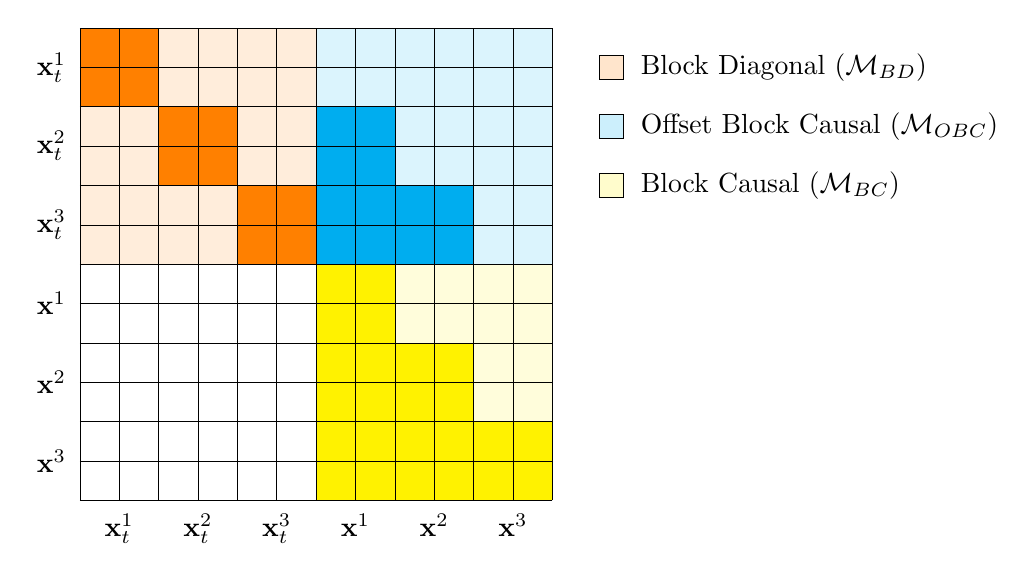
\begin{tikzpicture}[scale=0.5]
    % Grid
    % \draw[step=1cm,gray,very thin] (0,0) grid (12,12);

    % Block Diagonal
    \fill[orange!20, opacity=0.7] (0,12) rectangle (6,6);
    \foreach \i in {1,2,3}
    {
        \fill[orange] ({(\i-1)*2},{12-((\i-1)*2)}) rectangle ({(\i*2)},{12-(\i*2)});
    }

    % Block Causal Mask
    \fill[cyan!20, opacity=0.7] (6,12) rectangle (12,6);
    \fill[cyan] (6,10) rectangle (8,6);
    \fill[cyan] (8, 8) rectangle (10,6);

    % Block Causal for clean
    \fill[yellow!20, opacity=0.7] (6,6) rectangle (12,0);
    \fill[yellow] (6,6) rectangle (8,0);
    \fill[yellow] (8, 4) rectangle (10,0);
    \fill[yellow] (10, 2) rectangle (12,0);

    % Grid
    \draw[step=1cm,black,very thin] (0,0) grid (12,12);

    \foreach \x in {1, 3, 5}{
        \node[anchor=north] at (\x, -0.1) {$\mathbf{x}_t^{\pgfmathparse{int((\x/2)+1)}\pgfmathresult}$};
    }
    \foreach \x in {7, 9, 11}{
        \node[anchor=north] at (\x, -0.1) {$\mathbf{x}^{\pgfmathparse{int(((\x-6)/2)+1)}\pgfmathresult}$};
    }

    \foreach \y in {1, 3, 5}{
        \node[anchor=east] at (-0.1, 12-\y) {$\mathbf{x}_t^{\pgfmathparse{int((\y/2)+1)}\pgfmathresult}$};
    }
    \foreach \y in {7, 9, 11}{
        \node[anchor=east] at (-0.1, 12-\y) {$\mathbf{x}^{\pgfmathparse{int(((\y-6)/2)+1)}\pgfmathresult}$};
    }

    % Legend
    \node[draw, fill=orange!20, minimum width=0.3cm, minimum height=0.3cm] at (13.5, 11) {};
    \node[right] at (14, 11) {Block Diagonal ($\M_{BD}$)};
    
    \node[draw, fill=cyan!20, minimum width=0.3cm, minimum height=0.3cm] at (13.5, 9.5) {};
    \node[right] at (14, 9.5) {Offset Block Causal ($\M_{OBC}$)};
    
    \node[draw, fill=yellow!20, minimum width=0.3cm, minimum height=0.3cm] at (13.5, 8) {};
    \node[right] at (14, 8) {Block Causal ($\M_{BC}$)};

\end{tikzpicture}
\caption{Example of Specialized Attention Mask}
\label{fig:attention_mask_2}
\end{figure}


% \begin{python}

% # Define parameters
% seq_len = 128
% block_size = 16
% batch_size = 4
% num_heads = 8
% device = "cuda" if torch.cuda.is_available() else "cpu"

% # Create block mask
% my_block_diff_mask = partial(block_diff_mask, seq_len=seq_len, block_size=block_size)
% my_block_mask = create_block_mask(
%     my_block_diff_mask,
%     batch_size, num_heads, seq_len, seq_len, device=device, _compile=True
% )

% # **Single-Pass Flex Attention with Concatenated Sequence**
% @torch.compile(fullgraph=True, mode="max-autotune")
% def single_pass_block_diff_attn(q, k, v, block_mask):
%     return flex_attention(q, k, v, block_mask=block_mask)
% \end{python}



% \definecolor{ForestGreen}{RGB}{164,194,244}
% \definecolor{LightBlue}{RGB}{240,184,124}

% \begin{figure}[h]
% \centering
% \begin{tikzpicture}[scale=0.5]
%     % --- Colored Masks ---
%     % Draw each individual cell with white borders
%     \foreach \i in {0,...,5} {
%         \foreach \j in {0,...,5} {
%             \fill[white!20, draw=white] (\i,12-\j) rectangle (\i+1,11-\j);
%             \fill[white!20, draw=white] (\i+6,12-\j) rectangle (\i+7,11-\j);
%             \fill[white!20, draw=white] (\i+6,6-\j) rectangle (\i+7,5-\j);
%             \fill[white!20, draw=white] (\i,6-\j) rectangle (\i+1,5-\j);
%         }
%     }

%     % Block Diagonal (Upper-left)
%     \foreach \i in {1,2,3}{
%         \fill[LightBlue] ({(\i-1)*2},{12-((\i-1)*2)}) rectangle ({(\i*2)},{12-(\i*2)});
%     }

%     % Offset Block Causal (Upper-right)
%     \fill[ForestGreen] (6,10) rectangle (8,6);
%     \fill[ForestGreen] (8, 8) rectangle (10,6);

%     % Block Causal (Lower-right)
%     \fill[ForestGreen] (6,6) rectangle (8,0);
%     \fill[ForestGreen] (8, 4) rectangle (10,0);
%     \fill[ForestGreen] (10, 2) rectangle (12,0);


%     % Inner cell lines
%     \foreach \i in {1,...,5}{
%         \draw[white, thick] (\i,12) -- (\i,6);
%         \draw[white, thick] (\i+6,12) -- (\i+6,6);
%         \draw[white, thick] (\i,6) -- (\i,0);
%         \draw[white, thick] (\i+6,6) -- (\i+6,0);
%         \draw[white, thick] (0,12-\i) -- (6,12-\i);
%         \draw[white, thick] (6,12-\i) -- (12,12-\i);
%         \draw[white, thick] (0,6-\i) -- (6,6-\i);
%         \draw[white, thick] (6,6-\i) -- (12,6-\i);
%     }

%         % --- Quadrant Bounding Boxes ---
%     \draw[thick, black] (0,12) rectangle (6,6);    % Upper-left
%     \draw[thick, black] (6,12) rectangle (12,6);   % Upper-right
%     \draw[thick, black] (0,6) rectangle (6,0);     % Lower-left
%     \draw[thick, black] (6,6) rectangle (12,0);    % Lower-right


%     % Axis labels
%     \foreach \x in {1, 3, 5}{
%         \node[anchor=north] at (\x, -0.1) {$\mathbf{x}_t^{\pgfmathparse{int((\x/2)+1)}\pgfmathresult}$};
%     }
%     \foreach \x in {7, 9, 11}{
%         \node[anchor=north] at (\x, -0.1) {$\mathbf{x}^{\pgfmathparse{int(((\x-6)/2)+1)}\pgfmathresult}$};
%     }

%     \foreach \y in {1, 3, 5}{
%         \node[anchor=east] at (-0.1, 12-\y) {$\mathbf{x}_t^{\pgfmathparse{int((\y/2)+1)}\pgfmathresult}$};
%     }
%     \foreach \y in {7, 9, 11}{
%         \node[anchor=east] at (-0.1, 12-\y) {$\mathbf{x}^{\pgfmathparse{int(((\y-6)/2)+1)}\pgfmathresult}$};
%     }

% \end{tikzpicture}
% \caption{Example of Specialized Attention Mask with White Borders}
% \label{fig:attention_mask_quadrants_white}
% \end{figure}





% \begin{figure}[ht]
%   \centering
%   \includegraphics[width=0.8\textwidth]{figs/sar_graph.pdf}
%   \caption{Visualization of optimizing clipped noise schedules for training \algos{} on OWT. We plot the average masking rate used.}
%   \label{fig:nll_owt}
% \end{figure}

% \section{Ablations on training and sampling algorithms}
% \input{tables/abl_fwd_pass}
% \input{tables/abl_caching}

% \section{Sample vs. quality tradeoff}
% \begin{figure}[h]
%     \centering
%     \includegraphics[width=0.8\textwidth]{figs/nfesxgenppl.pdf}
%     \caption{Generative perplexities across number of function evaluations for generating 50 samples on OWT by varying $T\in\{100, 500, 1K, 5K, 10K, 50K\}$ in the reverse diffusion process. }
%     \label{fig:caching-wall-clock}
% \end{figure}

\subsection{Optimized Attention Kernel with FlexAttention}\label{suppl:flex-attention-kernels}

As ~\Cref{fig:attention_mask_2} demonstrates, our attention matrix is extremely sparse. We can exploit this sparsity to massively improve the efficiency of \algos{}.

FlexAttention~\citep{dong2024flex} is a compiler-driven programming model that enables efficient implementation of attention mechanisms with structured sparsity in PyTorch. It provides a flexible interface for defining custom attention masks while maintaining high performance comparable to manually optimized attention kernels.

Below in~\cref{fig:flex-attn-mask} we define a block-wise attention mask, \texttt{block\_diff\_mask}, based on its definition as $\M_{\text{full}} \in \{0, 1\}^{2L \times 2L}$ in Suppl. \ref{suppl:masks}. We fuse the attention operations into a single FlexAttention kernel designed to exploit the sparsity in our attention matrix to increase computational efficiency. By doing so, we perform the following optimizations:

\begin{itemize}
    \item \textbf{Precomputed Block Masking:} The \texttt{create\_block\_mask} utility generates a sparse attention mask at compile-time, avoiding per-step computation of invalid attention entries. Through sparsity-aware execution, FlexAttention kernels reduce the number of FLOPs in the attention computation.
    % \item \textbf{Causal and Cross-Block Attention:} Queries are restricted to attending within their designated blocks while allowing controlled cross-group attention, ensuring that dependencies are efficiently managed.
    \item \textbf{Reduced Memory Footprint:} By leveraging block-level sparsity, the attention mechanism avoids full materialization of large-scale attention matrices, significantly reducing memory overhead. FlexAttention minimizes memory accesses by skipping fully masked blocks.
    \item \textbf{Optimized Computation via \texttt{torch.compile}:} The integration of \texttt{torch.compile} enables kernel fusion and efficient execution on GPUs by generating optimized Triton-based kernels. This efficiently parallelizes masked attention computations using optimized GPU execution paths.
\end{itemize}

\begin{figure}
    \centering
    
\begin{minipage}{\linewidth}
\begin{python}
def block_diff_mask(b, h, q_idx, kv_idx, block_size, n):
    """
    Constructs the specialized block diffusion attention mask composed of three masks:
    - **Block Diagonal Mask (M_BD)**: Self-attention within noised blocks
    - **Offset Block Causal Mask (M_OBC)**: Cross-attention for conditional context
    - **Block Causal Mask (M_BC)**: Attention to update x0
    
    Args:
      b, h: Batch and head indices (ignored for mask logic).
      q_idx, kv_idx: Query and Key indices.
      block_size: Defines the block structure.
      n: Sequence length of x_0 and x_t

    
    Returns:
      A boolean attention mask.
    """
    
    # Indicate whether token belongs to xt (0) or x0 (1)
    x0_flag_q = (q_idx >= n)
    x0_flag_kv = (kv_idx >= n)
    
    # Compute block indices
    block_q = torch.where(x0_flag_q == 1,
                        (q_idx - n) // block_size,
                        q_idx // block_size)
    block_kv = torch.where(x0_flag_kv == 1,
                        (kv_idx - n) // block_size,
                        kv_idx // block_size)
    
    # **1. Block Diagonal Mask (M_BD) **
    block_diagonal = (block_q == block_kv) & (x0_flag_q == x0_flag_kv)
    
    # **2. Offset Block-Causal Mask (M_OBC) **
    offset_block_causal = (
        (block_q > block_kv)
        & (x0_flag_q == 0)
        & (x0_flag_kv == 1)
    )
    
    # **3. Block-Causal Mask (M_BC) **
    block_causal = (
        (block_q >= block_kv)
        & (x0_flag_q == 1)
        & (x0_flag_kv == 1)
    )
    
    # **4. Combine Masks **
    return block_diagonal | offset_block_causal | block_causal
    
\end{python}
\label{py::flex-attention}
\end{minipage}
    \caption{We can adapt the masking strategy from \cref{fig:attention_mask_2} to a FlexAttention compatible sparse masking function as above. This enables the creation of a customized JIT attention operation that uses significantly less memory with up to $\approx$5X speedup over the naive native scaled\_dot\_product\_attention implementation in PyTorch ($\geq$ 2.5) on a A5000 GPU with $L=1024$ and batch size $B=16$.}
    \label{fig:flex-attn-mask}
\end{figure}


\begin{figure}
    \centering
\begin{minipage}{\linewidth}
\begin{python}
from torch.nn.attention.flex_attention import flex_attention, create_block_mask
from functools import partial

# Define block-wise attention mask
my_block_diff_mask = partial(block_diff_mask, seq_len=seq_len, block_size=block_size)

# Generate optimized sparse block mask
block_mask = create_block_mask(my_block_diff_mask, None, None, seq_len*2, seq_len*2, device=device)

# Compute attention using FlexAttention
# Use no-cudagraphs to avoid an extra copy on small compile graphs. 
# Use max-autotune if compiling a larger model all at once.
@torch.compile(fullgraph=True, mode="max-autotune-no-cudagraphs")
def single_pass_block_diff_attn(q, k, v, block_mask):
    return flex_attention(q, k, v, block_mask=block_mask)
\end{python}
\end{minipage}
    \caption{Attention computation using FlexAttention with our proposed custom mask.}
\end{figure}



This implementation exploits FlexAttention's ability to dynamically optimize execution based on the provided sparsity pattern. By precomputing block-level sparsity and leveraging efficient kernel fusion, it enables scalable attention computation for long sequences.

% FlexAttention achieves superior performance by:

% \begin{itemize}
%     \item Reducing the number of FLOPs in attention computation through sparsity-aware execution.
%     \item Minimizing memory accesses by skipping fully sparse masked blocks.
%     \item Efficiently parallelizing masked attention computations using optimized GPU execution paths.
% \end{itemize}

Overall, this approach provides a principled method to accelerate attention computations while preserving structured dependency constraints. End-to-end, replacing FlashAttention kernels using a custom mask with FlexAttention kernels leads to $\approx15\%$ speedup in a model forward pass. We use a single A5000 for $L=1024$ and batch size $B=16$.
\newpage

\section{Experimental Details}
\label{suppl:details}
We closely follow the same training and evaluation setup as used by \citet{sahoo2024simple}. 

\subsection{Datasets}
\label{suppl:datasets}
We conduct experiments on two datasets: The One Billion Word Dataset (LM1B; \citet{chelba2014billion}) and OpenWebText (OWT; \citet{Gokaslan2019OpenWeb}). Models trained on LM1B use the \texttt{bert-base-uncased} tokenizer and a context length of 128. We report perplexities on the test split of LM1B. Models trained on OWT use the \texttt{GPT2} tokenizer \citet{radford2019language} and a context length of 1024. Since OWT does not have a validation split, we leave the last 100k documents for validation.

In preparing LM1B examples, \citet{sahoo2024simple} pad each example to fit in the context length of $L=128$ tokens. Since most examples consist of only a single sentence, block diffusion modeling for larger block sizes $L'>4$ would not be useful for training. Instead, we concatenate and wrap sequences to a length of 128. As a result, we retrain our autoregressive baseline, SEDD, and MDLM on LM1B with wrapping. 

Similarly for OWT, we do not pad or truncate sequences, but concatenate them and wrap them to a length of 1024 similar to LM1B. For unconditional generation experiments in Section \ref{subsec:samples}, we wish to generate sequences longer than the context length seen during training. However, \citet{sahoo2024simple} inject beginning-of-sequence and end-of-sequence tokens ([BOS], [EOS] respectively) at the beginning and end of the training context. Thus, baselines from~\citet{sahoo2024simple} will generate sequences that match the training context size. To examine model generations across varying lengths in Section \ref{subsec:samples}, we retrain our AR, SEDD, and MDLM baselines without injecting [BOS] and [EOS] tokens in the examples. We also adopt this preprocessing convention for training all \algos{} on OWT.

\subsection{Architecture}
\label{suppl:arch}
The model architecture augments the diffusion transformer \citep{peebles2023scalable} with rotary positional embeddings \citep{su2021roformer}. We parameterize our autoregressive baselines, SEDD, MDLM, and \algos{} with a transformer architecture from \citet{sahoo2024simple} that uses 12 layers, a hidden dimension of 768, and 12 attention heads. This corresponds to 110M parameters. We do not include timestep conditioning as \citet{sahoo2024simple} show it does not affect performance. We use the AdamW optimizer with a batch size of 512 and constant learning rate warmup from 0 to \texttt{3e-4} for 2.5K gradient updates.

\subsection{Training}
\label{suppl:training}
We train a base \algo{} using the maximum context length $L'=L$ for 850K gradient steps. Then, we fine-tune under varying $L'$ using the noise schedule optimization for 150K gradient steps on the One Billion Words dataset (LM1B) and OpenWebText (OWT). This translates to 65B tokens and 73 epochs on LM1B, 524B tokens and 60 epochs on OWT. We use 3090, A5000, A6000, and A100 GPUs.

\subsection{Likelihood Evaluation}
We use a single Monte Carlo estimate for sampling $t$ to evaluate the likelihood of a token block. We adopt a low-discrepancy sampler proposed in~\citet{kingma2021variational} that reduces the variance of this estimate by ensuring the time steps are more evenly spaced across the interval [0,1] following~\cite{sahoo2024simple}. In particular, we sample the time step for each block $b \in \{1, \dots, B\}$ and sequence $k \in \{1, \dots, K\}$ from a different partition of the uniform interval $t(k, b) \sim \mathcal{U}[ \frac{(k-1)B + b - 1}{KB}, \frac{(k-1)B + b}{KB} ]$. 

This low-discrepancy sampler is used for evaluation. For training, each masking probability may be sampled from a ``clipped" range $1 - \at \sim \mathcal{U}[\beta, \omega]$. During training, we uniformly sample $t \in [0, 1]$ under the low-discrepancy sampler. We then apply a linear interpolation to ensure that the masking probability is linear within the desired range: $1 - \at = \beta + (\omega - \beta) t$.

When reporting zero-shot likelihoods on benchmark datasets from~\citet{radford2019language} using models trained on OWT, we wrap all sequences to 1024 tokens and do not add [EOS] between sequences following~\citet{sahoo2024simple}.

\subsection{Inference}
\label{suppl:eval-details}
    \paragraph{Generative Perplexity}
    We report generative perplexity under GPT2-Large from models trained on OWT using a context length of 1024 tokens. Since GPT2-Large uses a context size of 1024, we compute the generative perplexity for samples longer than 1024 tokens using a sliding window with a stride length of 512 tokens. 

    \paragraph{Nucleus Sampling}
    Following SSD-LM \citep{han2022ssd}, we employ nucleus sampling for \algos{} and our baselines. For SSD-LM, we use their default hyperparameters $p=0.95$ for block size $L'=25$. For \algos{}, AR and MDLM, we use $p=0.9$. For SEDD, we find that $p=0.99$ works best.

     \paragraph{Number of Diffusion Steps} In Table \ref{tab:gen_ppl_2048}, \algos{} and MDLM use $T=5$K diffusion steps. \algos{} and MDLM use efficient sampling by caching the output of the denoising network as proposed by \citet{sahoo2024simple, ou2025your}, which ensures that the number of generation steps does not exceed the sample length $L$. Put simply, once a token is unmasked, it is never remasked as a result of the simplified denoising model (Suppl. \ref{supp:elbo}). We use MDLM's block-wise decoding algorithm for generating variable-length sequences, however these models are not trained with block diffusion. We adopt their default stride length of 512 tokens.
    
   SSD-LM (first row in Table \ref{tab:gen_ppl_2048}) and SEDD use $T=1$K diffusion steps. Since block diffusion performs $T$ diffusion steps for each block $b \in \{ 1, \dots, B \}$, SSD-LM undergoes $BT$ generation steps. Thus to fairly compare with SSD-LM, we also report generative perplexity for $T=25$ diffusion steps so that the number of generation steps does not exceed the sequence length (second row in Table \ref{tab:gen_ppl_2048}).

   \paragraph{Improved Categorical Sampling of Diffusion Models} We employ two improvements to Gumbel-based categorical sampling of diffusion models as proposed by~\citet{zheng2024masked}.
   
   First, we use the corrected Gumbel-based categorical sampling from \citet{zheng2024masked} by sampling 64-bit Gumbel variables. Reducing the precision to 32-bit has been shown to significantly truncate the Gumbel variables, lowering the temperature and decreasing the sentence entropy.
   
   Second, \citet{zheng2024masked} show that the MDLM sampling time scales with the diffusion steps $T$, even though the number of generation steps is bounded by the sequence length. For sample length $L$ and vocabulary size $V$, the sampler requires sampling $\mathcal{O}(T L V)$ uniform variables and performing logarithmic operations on them.
   
   We adopt the first-hitting sampler proposed by~\citet{zheng2024masked} that requires sampling $\mathcal{O}(L V)$ uniform variables, and thus greatly improves sampling speed especially when $T \gg L$. The first-hitting sampler is theoretically equivalent to the MDLM sampler and leverages two observations: (1) the transition probability is independent of the denoising network, (2) the transition probability is the same for all masked tokens for a given $t$. Thus, the first timestep where a token is unmasked can be analytically sampled as follows (assuming a linear schedule where $\at = 1 - t$):
   \begin{align}
       t_{n-1} = t_n u^{1 / n},
   \end{align}
   \noindent where $n \in \{ L, \dots, 1\}$ denotes the number of masked tokens, $u_n \sim \mathcal{U}[0,1]$ and $t_{n-1}$ corresponds to the first timestep where $n-1$ tokens are masked.

    \paragraph{Variable-Length Sequence Generation}
    For arbitrary-length sequence generation using \algos{} and AR in Table \ref{tab:owt-gen-lens}, we continue to sample tokens until the following stopping criteria are met: 
    \begin{enumerate}
        \item an [EOS] token is sampled
        % \item the average likelihood of the last 256-token chunk is below 0.1
        \item the average entropy of the the last 256-token chunk is below 4
    \end{enumerate}
    \noindent where criterion 2 are necessary to prevent run-on samples from compounding errors (for example, a sequence of repeating tokens). We find that degenerate samples with low entropy result in significantly low perplexities under \texttt{GPT2} and lower the reported generative perplexity. Thus, when a sample meets criterion 2, we regenerate the sample when reporting generative perplexity in Table \ref{tab:gen_ppl_2048}.
\section{Samples}\label{suppl:summaries}
\input{samples/mdlm_samps}
\newpage
\input{samples/sar_samps}
\newpage
\input{samples/ar_samps}


% \input{tables/variances_owt}
% \input{tables/variances_text8}

% \section{Experimental details}


% \subsection{OpenWebText}

% \subsection{CNN/DailyMail


\end{document}
